\documentclass[twoside]{book}

% Packages required by doxygen
\usepackage{fixltx2e}
\usepackage{calc}
\usepackage{doxygen}
\usepackage[export]{adjustbox} % also loads graphicx
\usepackage{graphicx}
\usepackage[utf8]{inputenc}
\usepackage{makeidx}
\usepackage{multicol}
\usepackage{multirow}
\PassOptionsToPackage{warn}{textcomp}
\usepackage{textcomp}
\usepackage[nointegrals]{wasysym}
\usepackage[table]{xcolor}

% Font selection
\usepackage[T1]{fontenc}
\usepackage[scaled=.90]{helvet}
\usepackage{courier}
\usepackage{amssymb}
\usepackage{sectsty}
\renewcommand{\familydefault}{\sfdefault}
\allsectionsfont{%
  \fontseries{bc}\selectfont%
  \color{darkgray}%
}
\renewcommand{\DoxyLabelFont}{%
  \fontseries{bc}\selectfont%
  \color{darkgray}%
}
\newcommand{\+}{\discretionary{\mbox{\scriptsize$\hookleftarrow$}}{}{}}

% Page & text layout
\usepackage{geometry}
\geometry{%
  a4paper,%
  top=2.5cm,%
  bottom=2.5cm,%
  left=2.5cm,%
  right=2.5cm%
}
\tolerance=750
\hfuzz=15pt
\hbadness=750
\setlength{\emergencystretch}{15pt}
\setlength{\parindent}{0cm}
\setlength{\parskip}{3ex plus 2ex minus 2ex}
\makeatletter
\renewcommand{\paragraph}{%
  \@startsection{paragraph}{4}{0ex}{-1.0ex}{1.0ex}{%
    \normalfont\normalsize\bfseries\SS@parafont%
  }%
}
\renewcommand{\subparagraph}{%
  \@startsection{subparagraph}{5}{0ex}{-1.0ex}{1.0ex}{%
    \normalfont\normalsize\bfseries\SS@subparafont%
  }%
}
\makeatother

% Headers & footers
\usepackage{fancyhdr}
\pagestyle{fancyplain}
\fancyhead[LE]{\fancyplain{}{\bfseries\thepage}}
\fancyhead[CE]{\fancyplain{}{}}
\fancyhead[RE]{\fancyplain{}{\bfseries\leftmark}}
\fancyhead[LO]{\fancyplain{}{\bfseries\rightmark}}
\fancyhead[CO]{\fancyplain{}{}}
\fancyhead[RO]{\fancyplain{}{\bfseries\thepage}}
\fancyfoot[LE]{\fancyplain{}{}}
\fancyfoot[CE]{\fancyplain{}{}}
\fancyfoot[RE]{\fancyplain{}{\bfseries\scriptsize 制作者 Doxygen }}
\fancyfoot[LO]{\fancyplain{}{\bfseries\scriptsize 制作者 Doxygen }}
\fancyfoot[CO]{\fancyplain{}{}}
\fancyfoot[RO]{\fancyplain{}{}}
\renewcommand{\footrulewidth}{0.4pt}
\renewcommand{\chaptermark}[1]{%
  \markboth{#1}{}%
}
\renewcommand{\sectionmark}[1]{%
  \markright{\thesection\ #1}%
}

% Indices & bibliography
\usepackage{natbib}
\usepackage[titles]{tocloft}
\setcounter{tocdepth}{3}
\setcounter{secnumdepth}{5}
\makeindex

% Hyperlinks (required, but should be loaded last)
\usepackage{ifpdf}
\ifpdf
  \usepackage[pdftex,pagebackref=true]{hyperref}
\else
  \usepackage[ps2pdf,pagebackref=true]{hyperref}
\fi
\hypersetup{%
  colorlinks=true,%
  linkcolor=blue,%
  citecolor=blue,%
  unicode%
}

% Custom commands
\newcommand{\clearemptydoublepage}{%
  \newpage{\pagestyle{empty}\cleardoublepage}%
}

\usepackage{caption}
\captionsetup{labelsep=space,justification=centering,font={bf},singlelinecheck=off,skip=4pt,position=top}

%===== C O N T E N T S =====

\begin{document}

% Titlepage & ToC
\hypersetup{pageanchor=false,
             bookmarksnumbered=true,
             pdfencoding=unicode
            }
\pagenumbering{alph}
\begin{titlepage}
\vspace*{7cm}
\begin{center}%
{\Large Kerbal \\[1ex]\large 1.\+0 }\\
\vspace*{1cm}
{\large 制作者 Doxygen 1.8.13}\\
\end{center}
\end{titlepage}
\clearemptydoublepage
\pagenumbering{roman}
\tableofcontents
\clearemptydoublepage
\pagenumbering{arabic}
\hypersetup{pageanchor=true}

%--- Begin generated contents ---
\chapter{命名空间索引}
\section{命名空间列表}
这里列出了所有文档化的命名空间定义,附带简要说明\+:\begin{DoxyCompactList}
\item\contentsline{section}{\hyperlink{namespacekerbal}{kerbal} \\*Kerbal 库 }{\pageref{namespacekerbal}}{}
\item\contentsline{section}{\hyperlink{namespacekerbal_1_1math}{kerbal\+::math} \\*数学计算子库 }{\pageref{namespacekerbal_1_1math}}{}
\item\contentsline{section}{\hyperlink{namespacekerbal_1_1math_1_1complexor}{kerbal\+::math\+::complexor} \\*向量计算子库 }{\pageref{namespacekerbal_1_1math_1_1complexor}}{}
\item\contentsline{section}{\hyperlink{namespacekerbal_1_1math_1_1matrix}{kerbal\+::math\+::matrix} \\*矩阵计算子库 }{\pageref{namespacekerbal_1_1math_1_1matrix}}{}
\end{DoxyCompactList}

\chapter{继承关系索引}
\section{类继承关系}
此继承关系列表按字典顺序粗略的排序\+: \begin{DoxyCompactList}
\item \contentsline{section}{kerbal\+:\+:data\+\_\+struct\+:\+:array\+\_\+2d\+:\+:Array\+\_\+2d$<$ Type $>$}{\pageref{classkerbal_1_1data__struct_1_1array__2d_1_1_array__2d}}{}
\item \contentsline{section}{kerbal\+:\+:data\+\_\+struct\+:\+:array\+\_\+2d\+:\+:Array\+\_\+2d$<$ double $>$}{\pageref{classkerbal_1_1data__struct_1_1array__2d_1_1_array__2d}}{}
\begin{DoxyCompactList}
\item \contentsline{section}{kerbal\+:\+:math\+:\+:matrix\+:\+:Matrix}{\pageref{classkerbal_1_1math_1_1matrix_1_1_matrix}}{}
\end{DoxyCompactList}
\item \contentsline{section}{kerbal\+:\+:math\+:\+:complex\+:\+:Complex}{\pageref{classkerbal_1_1math_1_1complex_1_1_complex}}{}
\item \contentsline{section}{kerbal\+:\+:math\+:\+:complexor\+:\+:Complexor$<$ Type $>$}{\pageref{classkerbal_1_1math_1_1complexor_1_1_complexor}}{}
\item \contentsline{section}{kerbal\+:\+:utility\+:\+:dbstream\+:\+:Dbstream}{\pageref{classkerbal_1_1utility_1_1dbstream_1_1_dbstream}}{}
\item exception\begin{DoxyCompactList}
\item \contentsline{section}{kerbal\+:\+:traceable\+:\+:Tr\+\_\+except}{\pageref{classkerbal_1_1traceable_1_1_tr__except}}{}
\end{DoxyCompactList}
\item \contentsline{section}{Object}{\pageref{class_object}}{}
\item \contentsline{section}{kerbal\+:\+:Range\+:\+:Range\+\_\+view\+:\+:Range\+\_\+iterator}{\pageref{classkerbal_1_1_range_1_1_range__view_1_1_range__iterator}}{}
\item \contentsline{section}{kerbal\+:\+:Range\+:\+:Range\+\_\+view}{\pageref{classkerbal_1_1_range_1_1_range__view}}{}
\item \contentsline{section}{kerbal\+:\+:data\+\_\+struct\+:\+:array\+\_\+2d\+:\+:safety$<$ Type $>$}{\pageref{classkerbal_1_1data__struct_1_1array__2d_1_1safety}}{}
\item \contentsline{section}{kerbal\+:\+:spherical\+:\+:Spherical}{\pageref{classkerbal_1_1spherical_1_1_spherical}}{}
\item \contentsline{section}{kerbal\+:\+:traceable\+:\+:Tr\+\_\+except\+:\+:Trace}{\pageref{structkerbal_1_1traceable_1_1_tr__except_1_1_trace}}{}
\end{DoxyCompactList}

\chapter{类索引}
\section{类列表}
这里列出了所有类、结构、联合以及接口定义等,并附带简要说明\+:\begin{DoxyCompactList}
\item\contentsline{section}{\hyperlink{classarray__2d_1_1_array__2d}{array\+\_\+2d\+::\+Array\+\_\+2d$<$ Type $>$} \\*动态二维数组类 }{\pageref{classarray__2d_1_1_array__2d}}{}
\item\contentsline{section}{\hyperlink{classkerbal_1_1math_1_1_complex}{kerbal\+::math\+::\+Complex} }{\pageref{classkerbal_1_1math_1_1_complex}}{}
\item\contentsline{section}{\hyperlink{classkerbal_1_1math_1_1_complexor}{kerbal\+::math\+::\+Complexor$<$ Type $>$} }{\pageref{classkerbal_1_1math_1_1_complexor}}{}
\item\contentsline{section}{\hyperlink{classkerbal_1_1utility_1_1dbstream_1_1_dbstream}{kerbal\+::utility\+::dbstream\+::\+Dbstream} }{\pageref{classkerbal_1_1utility_1_1dbstream_1_1_dbstream}}{}
\item\contentsline{section}{\hyperlink{classkerbal_1_1math_1_1_matrix}{kerbal\+::math\+::\+Matrix} \\*矩阵类 }{\pageref{classkerbal_1_1math_1_1_matrix}}{}
\item\contentsline{section}{\hyperlink{class_object}{Object} }{\pageref{class_object}}{}
\item\contentsline{section}{\hyperlink{classarray__2d_1_1safety}{array\+\_\+2d\+::safety$<$ Type $>$} \\*动态二维数组类的安全下标类 }{\pageref{classarray__2d_1_1safety}}{}
\item\contentsline{section}{\hyperlink{classkerbal_1_1spherical_1_1_spherical}{kerbal\+::spherical\+::\+Spherical} }{\pageref{classkerbal_1_1spherical_1_1_spherical}}{}
\item\contentsline{section}{\hyperlink{classkerbal_1_1traceable_1_1_tr__except}{kerbal\+::traceable\+::\+Tr\+\_\+except} }{\pageref{classkerbal_1_1traceable_1_1_tr__except}}{}
\item\contentsline{section}{\hyperlink{structkerbal_1_1traceable_1_1_tr__except_1_1_trace}{kerbal\+::traceable\+::\+Tr\+\_\+except\+::\+Trace} }{\pageref{structkerbal_1_1traceable_1_1_tr__except_1_1_trace}}{}
\end{DoxyCompactList}

\chapter{文件索引}
\section{文件列表}
这里列出了所有文档化的文件,并附带简要说明\+:\begin{DoxyCompactList}
\item\contentsline{section}{src/kerbal/{\bfseries array\+\_\+2d.\+hpp} }{\pageref{array__2d_8hpp}}{}
\item\contentsline{section}{src/kerbal/{\bfseries array\+\_\+2d\+\_\+base.\+hpp} }{\pageref{array__2d__base_8hpp}}{}
\item\contentsline{section}{src/kerbal/{\bfseries array\+\_\+serve.\+hpp} }{\pageref{array__serve_8hpp}}{}
\item\contentsline{section}{src/kerbal/{\bfseries choose.\+hpp} }{\pageref{choose_8hpp}}{}
\item\contentsline{section}{src/kerbal/{\bfseries dbstream.\+hpp} }{\pageref{dbstream_8hpp}}{}
\item\contentsline{section}{src/kerbal/{\bfseries except\+\_\+\+C++0x.\+hpp} }{\pageref{except___c_09_090x_8hpp}}{}
\item\contentsline{section}{src/kerbal/{\bfseries exe\+\_\+serve.\+hpp} }{\pageref{exe__serve_8hpp}}{}
\item\contentsline{section}{src/kerbal/{\bfseries range.\+hpp} }{\pageref{range_8hpp}}{}
\item\contentsline{section}{src/kerbal/{\bfseries sort.\+hpp} }{\pageref{sort_8hpp}}{}
\item\contentsline{section}{src/kerbal/{\bfseries sort\+\_\+base.\+hpp} }{\pageref{sort__base_8hpp}}{}
\item\contentsline{section}{src/kerbal/{\bfseries Spherical.\+hpp} }{\pageref{_spherical_8hpp}}{}
\item\contentsline{section}{src/kerbal/{\bfseries string\+\_\+serve.\+hpp} }{\pageref{string__serve_8hpp}}{}
\item\contentsline{section}{src/kerbal/{\bfseries tick\+\_\+count.\+h} }{\pageref{tick__count_8h}}{}
\item\contentsline{section}{src/kerbal/{\bfseries Trexcept.\+hpp} }{\pageref{_trexcept_8hpp}}{}
\item\contentsline{section}{src/kerbal/math/{\bfseries basic\+\_\+math.\+hpp} }{\pageref{basic__math_8hpp}}{}
\item\contentsline{section}{src/kerbal/math/{\bfseries complex.\+hpp} }{\pageref{complex_8hpp}}{}
\item\contentsline{section}{src/kerbal/math/{\bfseries complexor.\+hpp} }{\pageref{complexor_8hpp}}{}
\item\contentsline{section}{src/kerbal/math/{\bfseries complexor\+\_\+base.\+hpp} }{\pageref{complexor__base_8hpp}}{}
\item\contentsline{section}{src/kerbal/math/{\bfseries integral.\+hpp} }{\pageref{integral_8hpp}}{}
\item\contentsline{section}{src/kerbal/math/{\bfseries mapminmax.\+hpp} }{\pageref{mapminmax_8hpp}}{}
\item\contentsline{section}{src/kerbal/math/\hyperlink{matrix_8hpp}{matrix.\+hpp} \\*本文件提供了对基本矩阵计算的支持 }{\pageref{matrix_8hpp}}{}
\item\contentsline{section}{src/kerbal/math/{\bfseries omp\+\_\+settings.\+hpp} }{\pageref{omp__settings_8hpp}}{}
\item\contentsline{section}{src/kerbal/math/{\bfseries randnum.\+hpp} }{\pageref{randnum_8hpp}}{}
\item\contentsline{section}{src/kerbal/math/{\bfseries statistics.\+hpp} }{\pageref{statistics_8hpp}}{}
\end{DoxyCompactList}

\chapter{命名空间文档}
\hypertarget{namespacekerbal}{}\section{kerbal 命名空间参考}
\label{namespacekerbal}\index{kerbal@{kerbal}}


kerbal 库  


\subsection*{命名空间}
\begin{DoxyCompactItemize}
\item 
 \hyperlink{namespacekerbal_1_1math}{math}
\begin{DoxyCompactList}\small\item\em 数学计算子库 \end{DoxyCompactList}\end{DoxyCompactItemize}


\subsection{详细描述}
kerbal 库 

\begin{DoxyAuthor}{作者}
倪文卿 
\end{DoxyAuthor}

\hypertarget{namespacekerbal_1_1math}{}\section{kerbal\+:\+:math 命名空间参考}
\label{namespacekerbal_1_1math}\index{kerbal\+::math@{kerbal\+::math}}


数学计算子库  


\subsection*{命名空间}
\begin{DoxyCompactItemize}
\item 
 \hyperlink{namespacekerbal_1_1math_1_1complexor}{complexor}
\begin{DoxyCompactList}\small\item\em 向量计算子库 \end{DoxyCompactList}\item 
 \hyperlink{namespacekerbal_1_1math_1_1matrix}{matrix}
\begin{DoxyCompactList}\small\item\em 矩阵计算子库 \end{DoxyCompactList}\end{DoxyCompactItemize}


\subsection{详细描述}
数学计算子库 
\chapter{类说明}
\hypertarget{classarray__2d_1_1_array__2d}{}\section{array\+\_\+2d\+:\+:Array\+\_\+2d$<$ Type $>$ 模板类 参考}
\label{classarray__2d_1_1_array__2d}\index{array\+\_\+2d\+::\+Array\+\_\+2d$<$ Type $>$@{array\+\_\+2d\+::\+Array\+\_\+2d$<$ Type $>$}}


动态二维数组类  




{\ttfamily \#include $<$array\+\_\+2d.\+hpp$>$}

\subsection*{Public 类型}
\begin{DoxyCompactItemize}
\item 
\mbox{\Hypertarget{classarray__2d_1_1_array__2d_a71a2f6542c925b3851cf79ce7ffd3439}\label{classarray__2d_1_1_array__2d_a71a2f6542c925b3851cf79ce7ffd3439}} 
enum {\bfseries print\+\_\+style} \{ {\bfseries frame\+\_\+with\+\_\+corner}, 
{\bfseries frame\+\_\+only}, 
{\bfseries none}
 \}
\end{DoxyCompactItemize}
\subsection*{Public 成员函数}
\begin{DoxyCompactItemize}
\item 
\hyperlink{classarray__2d_1_1_array__2d_a46091ff0390e83377efa1d2b9e9870d5}{Array\+\_\+2d} ()  throw ()
\begin{DoxyCompactList}\small\item\em 构造一个 0 行 0 列的空二维数组 \end{DoxyCompactList}\item 
\hyperlink{classarray__2d_1_1_array__2d_ae1230f7ac7f0558df988369c47ef78ba}{Array\+\_\+2d} (const int \hyperlink{classarray__2d_1_1_array__2d_a17b90b53a8e0002452e96c2b7f74820b}{row}, const int \hyperlink{classarray__2d_1_1_array__2d_abdf56a1c0f22088353d9a32de9680d76}{column})
\begin{DoxyCompactList}\small\item\em 构造一个 row 行 column 列的二维数组, 数组中每个元素的初始值由默认构造函数生成 \end{DoxyCompactList}\item 
\hyperlink{classarray__2d_1_1_array__2d_aae6ad90ad3b5f3549be4df81a8559ef6}{Array\+\_\+2d} (const int \hyperlink{classarray__2d_1_1_array__2d_a17b90b53a8e0002452e96c2b7f74820b}{row}, const int \hyperlink{classarray__2d_1_1_array__2d_abdf56a1c0f22088353d9a32de9680d76}{column}, const Type \&val)
\begin{DoxyCompactList}\small\item\em 构造一个 row 行 column 列的二维数组, 数组中每个元素的初始值由参数 val 指定 \end{DoxyCompactList}\item 
\hyperlink{classarray__2d_1_1_array__2d_ae7e62c74794fd2ccc4c3923cf0ae2e41}{Array\+\_\+2d} (Type($\ast$function)(), const int \hyperlink{classarray__2d_1_1_array__2d_a17b90b53a8e0002452e96c2b7f74820b}{row}, const int \hyperlink{classarray__2d_1_1_array__2d_abdf56a1c0f22088353d9a32de9680d76}{column}, bool para)
\item 
\mbox{\Hypertarget{classarray__2d_1_1_array__2d_a5465e7ab30fa80206308a9a7c76571a7}\label{classarray__2d_1_1_array__2d_a5465e7ab30fa80206308a9a7c76571a7}} 
{\bfseries Array\+\_\+2d} (Type($\ast$function)(int, int), const int \hyperlink{classarray__2d_1_1_array__2d_a17b90b53a8e0002452e96c2b7f74820b}{row}, const int \hyperlink{classarray__2d_1_1_array__2d_abdf56a1c0f22088353d9a32de9680d76}{column}, bool para)
\item 
\mbox{\Hypertarget{classarray__2d_1_1_array__2d_ae7bbc97860822dbdc333d61c92c3e111}\label{classarray__2d_1_1_array__2d_ae7bbc97860822dbdc333d61c92c3e111}} 
{\footnotesize template$<$size\+\_\+t M, size\+\_\+t N$>$ }\\{\bfseries Array\+\_\+2d} (const Type(\&src)\mbox{[}M\mbox{]}\mbox{[}N\mbox{]}, const int \hyperlink{classarray__2d_1_1_array__2d_a17b90b53a8e0002452e96c2b7f74820b}{row}, const int \hyperlink{classarray__2d_1_1_array__2d_abdf56a1c0f22088353d9a32de9680d76}{column})
\item 
\mbox{\Hypertarget{classarray__2d_1_1_array__2d_abeeaa67b7ad1287747e154e78a5720d5}\label{classarray__2d_1_1_array__2d_abeeaa67b7ad1287747e154e78a5720d5}} 
{\bfseries Array\+\_\+2d} (const Type arr\mbox{[}$\,$\mbox{]}, int len, bool in\+\_\+a\+\_\+row=true)
\item 
\mbox{\Hypertarget{classarray__2d_1_1_array__2d_a82566af7cfdef956f9b6029321f6ee00}\label{classarray__2d_1_1_array__2d_a82566af7cfdef956f9b6029321f6ee00}} 
{\bfseries Array\+\_\+2d} (const \hyperlink{classarray__2d_1_1_array__2d}{Array\+\_\+2d} \&src)
\item 
bool \hyperlink{classarray__2d_1_1_array__2d_a5c22f2f9e9c2aa9436aecb14dab6b27d}{empty} () const  throw ()
\begin{DoxyCompactList}\small\item\em 查询动态二维数组是否为空数组 \end{DoxyCompactList}\item 
\mbox{\Hypertarget{classarray__2d_1_1_array__2d_aa72a614483a59ce37170c4b5bc75b1b1}\label{classarray__2d_1_1_array__2d_aa72a614483a59ce37170c4b5bc75b1b1}} 
void \hyperlink{classarray__2d_1_1_array__2d_aa72a614483a59ce37170c4b5bc75b1b1}{clear} ()  throw ()
\begin{DoxyCompactList}\small\item\em 将动态二维数组置为空数组 \end{DoxyCompactList}\item 
\mbox{\Hypertarget{classarray__2d_1_1_array__2d_afcb670f03ddb8b39e9fb8d6120bf736b}\label{classarray__2d_1_1_array__2d_afcb670f03ddb8b39e9fb8d6120bf736b}} 
void {\bfseries resize} (int new\+\_\+row, int new\+\_\+column)
\item 
int \hyperlink{classarray__2d_1_1_array__2d_aa2ac561244188718d0c1ee14568b772e}{get\+\_\+row} () const
\begin{DoxyCompactList}\small\item\em 获取动态二维数组的行数 \end{DoxyCompactList}\item 
\mbox{\Hypertarget{classarray__2d_1_1_array__2d_a4754750259b7e261eb84c50fce26a42f}\label{classarray__2d_1_1_array__2d_a4754750259b7e261eb84c50fce26a42f}} 
int {\bfseries get\+\_\+column} () const
\item 
\mbox{\Hypertarget{classarray__2d_1_1_array__2d_acc2e1e42f604d7e4d659c255fb166264}\label{classarray__2d_1_1_array__2d_acc2e1e42f604d7e4d659c255fb166264}} 
const Type $\ast$$\ast$ {\bfseries get\+\_\+data} () const
\item 
\mbox{\Hypertarget{classarray__2d_1_1_array__2d_ac5c501e9853106e7fe829cf010dbd1cc}\label{classarray__2d_1_1_array__2d_ac5c501e9853106e7fe829cf010dbd1cc}} 
bool {\bfseries is\+\_\+const} ()
\item 
\mbox{\Hypertarget{classarray__2d_1_1_array__2d_a9d70a21f470c0bafd844f03483675c0b}\label{classarray__2d_1_1_array__2d_a9d70a21f470c0bafd844f03483675c0b}} 
bool {\bfseries is\+\_\+const} () const
\item 
\mbox{\Hypertarget{classarray__2d_1_1_array__2d_a7915b02b6dae8959e527da8b780b3d4f}\label{classarray__2d_1_1_array__2d_a7915b02b6dae8959e527da8b780b3d4f}} 
Type \& {\bfseries get} (int \hyperlink{classarray__2d_1_1_array__2d_a17b90b53a8e0002452e96c2b7f74820b}{row}, int \hyperlink{classarray__2d_1_1_array__2d_abdf56a1c0f22088353d9a32de9680d76}{column})  throw (std\+::out\+\_\+of\+\_\+range)
\item 
\mbox{\Hypertarget{classarray__2d_1_1_array__2d_add9e517d2162ff5de4927171a185dee9}\label{classarray__2d_1_1_array__2d_add9e517d2162ff5de4927171a185dee9}} 
const Type \& {\bfseries get} (int \hyperlink{classarray__2d_1_1_array__2d_a17b90b53a8e0002452e96c2b7f74820b}{row}, int \hyperlink{classarray__2d_1_1_array__2d_abdf56a1c0f22088353d9a32de9680d76}{column}) const  throw (std\+::out\+\_\+of\+\_\+range)
\item 
\mbox{\Hypertarget{classarray__2d_1_1_array__2d_a0ebf20317d3f8a6c1b58634b387ca0ed}\label{classarray__2d_1_1_array__2d_a0ebf20317d3f8a6c1b58634b387ca0ed}} 
void {\bfseries set} (int \hyperlink{classarray__2d_1_1_array__2d_a17b90b53a8e0002452e96c2b7f74820b}{row}, int \hyperlink{classarray__2d_1_1_array__2d_abdf56a1c0f22088353d9a32de9680d76}{column}, const Type \&value)  throw (std\+::out\+\_\+of\+\_\+range)
\item 
\mbox{\Hypertarget{classarray__2d_1_1_array__2d_a287f572e2ecf5041e04b0c93dbad60ef}\label{classarray__2d_1_1_array__2d_a287f572e2ecf5041e04b0c93dbad60ef}} 
{\footnotesize template$<$class T $>$ }\\void {\bfseries set} (const T src\mbox{[}$\,$\mbox{]}, int \hyperlink{classarray__2d_1_1_array__2d_a17b90b53a8e0002452e96c2b7f74820b}{row}, int \hyperlink{classarray__2d_1_1_array__2d_abdf56a1c0f22088353d9a32de9680d76}{column})
\item 
\mbox{\Hypertarget{classarray__2d_1_1_array__2d_ae4b288551d0af6885bbf4fa6430397dd}\label{classarray__2d_1_1_array__2d_ae4b288551d0af6885bbf4fa6430397dd}} 
void {\bfseries do\+\_\+call} (Type($\ast$\+\_\+\+\_\+pf)(Type))
\item 
\mbox{\Hypertarget{classarray__2d_1_1_array__2d_a1f793af35dd704bcfa9e459003a97ac9}\label{classarray__2d_1_1_array__2d_a1f793af35dd704bcfa9e459003a97ac9}} 
void {\bfseries do\+\_\+call} (Type($\ast$\+\_\+\+\_\+pf)(int, int))
\item 
\mbox{\Hypertarget{classarray__2d_1_1_array__2d_a38723633d1e7f945b830a305b5199c5c}\label{classarray__2d_1_1_array__2d_a38723633d1e7f945b830a305b5199c5c}} 
void {\bfseries do\+\_\+call} (Type($\ast$\+\_\+\+\_\+pf)(Type, int, int))
\item 
\mbox{\Hypertarget{classarray__2d_1_1_array__2d_ab6ea27aa8e2caf13ed22b601d2b12871}\label{classarray__2d_1_1_array__2d_ab6ea27aa8e2caf13ed22b601d2b12871}} 
const \hyperlink{classarray__2d_1_1_array__2d}{Array\+\_\+2d}$<$ Type $>$ {\bfseries call\+\_\+of} (Type($\ast$\+\_\+\+\_\+pf)(Type)) const
\item 
\mbox{\Hypertarget{classarray__2d_1_1_array__2d_af5719e0fea6efee80a750404367c184a}\label{classarray__2d_1_1_array__2d_af5719e0fea6efee80a750404367c184a}} 
const \hyperlink{classarray__2d_1_1_array__2d}{Array\+\_\+2d}$<$ Type $>$ {\bfseries call\+\_\+of} (Type($\ast$\+\_\+\+\_\+pf)(int, int)) const
\item 
\mbox{\Hypertarget{classarray__2d_1_1_array__2d_ab0296eaf3e67454587b361a7e51760da}\label{classarray__2d_1_1_array__2d_ab0296eaf3e67454587b361a7e51760da}} 
const \hyperlink{classarray__2d_1_1_array__2d}{Array\+\_\+2d}$<$ Type $>$ {\bfseries call\+\_\+of} (Type($\ast$\+\_\+\+\_\+pf)(Type, int, int)) const
\item 
\mbox{\Hypertarget{classarray__2d_1_1_array__2d_a1a8bc1db397a592a7d1f99bc989675ba}\label{classarray__2d_1_1_array__2d_a1a8bc1db397a592a7d1f99bc989675ba}} 
{\footnotesize template$<$print\+\_\+style print\+\_\+frame = frame\+\_\+with\+\_\+corner$>$ }\\void {\bfseries print} (std\+::ostream \&output=std\+::cout) const
\item 
\mbox{\Hypertarget{classarray__2d_1_1_array__2d_a59886ee3e61eb4cadde05708ce53cc34}\label{classarray__2d_1_1_array__2d_a59886ee3e61eb4cadde05708ce53cc34}} 
\hyperlink{classarray__2d_1_1safety}{safety}$<$ Type $>$ {\bfseries operator\mbox{[}$\,$\mbox{]}} (int \hyperlink{classarray__2d_1_1_array__2d_a17b90b53a8e0002452e96c2b7f74820b}{row})  throw (std\+::out\+\_\+of\+\_\+range)
\item 
\mbox{\Hypertarget{classarray__2d_1_1_array__2d_a0ae4fba64e3bf45dfbf32bf9694f5ccd}\label{classarray__2d_1_1_array__2d_a0ae4fba64e3bf45dfbf32bf9694f5ccd}} 
const \hyperlink{classarray__2d_1_1safety}{safety}$<$ Type $>$ {\bfseries operator\mbox{[}$\,$\mbox{]}} (int \hyperlink{classarray__2d_1_1_array__2d_a17b90b53a8e0002452e96c2b7f74820b}{row}) const  throw (std\+::out\+\_\+of\+\_\+range)
\item 
\mbox{\Hypertarget{classarray__2d_1_1_array__2d_a475a57fdcb88319f7fc794e898dcd85e}\label{classarray__2d_1_1_array__2d_a475a57fdcb88319f7fc794e898dcd85e}} 
Type \& {\bfseries operator()} (int \hyperlink{classarray__2d_1_1_array__2d_a17b90b53a8e0002452e96c2b7f74820b}{row}, int \hyperlink{classarray__2d_1_1_array__2d_abdf56a1c0f22088353d9a32de9680d76}{column})  throw (std\+::out\+\_\+of\+\_\+range)
\item 
\mbox{\Hypertarget{classarray__2d_1_1_array__2d_afe5d62c7acaf8b69ba72ec83c04263b2}\label{classarray__2d_1_1_array__2d_afe5d62c7acaf8b69ba72ec83c04263b2}} 
const Type \& {\bfseries operator()} (int \hyperlink{classarray__2d_1_1_array__2d_a17b90b53a8e0002452e96c2b7f74820b}{row}, int \hyperlink{classarray__2d_1_1_array__2d_abdf56a1c0f22088353d9a32de9680d76}{column}) const  throw (std\+::out\+\_\+of\+\_\+range)
\item 
\mbox{\Hypertarget{classarray__2d_1_1_array__2d_a8e69d517057b9beaffa6fe0469df7785}\label{classarray__2d_1_1_array__2d_a8e69d517057b9beaffa6fe0469df7785}} 
virtual size\+\_\+t {\bfseries get\+\_\+digit\+\_\+size} () const
\item 
\mbox{\Hypertarget{classarray__2d_1_1_array__2d_a77b3c52e832f2c288df90b7ed2c78e83}\label{classarray__2d_1_1_array__2d_a77b3c52e832f2c288df90b7ed2c78e83}} 
virtual void {\bfseries test\+\_\+row} (const int row\+\_\+test) const  throw (std\+::out\+\_\+of\+\_\+range)
\item 
\mbox{\Hypertarget{classarray__2d_1_1_array__2d_a2a507f8ce013c7dc51cc919c6d5fc015}\label{classarray__2d_1_1_array__2d_a2a507f8ce013c7dc51cc919c6d5fc015}} 
virtual void {\bfseries test\+\_\+column} (const int column\+\_\+test) const  throw (std\+::out\+\_\+of\+\_\+range)
\item 
\mbox{\Hypertarget{classarray__2d_1_1_array__2d_a335a5d4d3d50f0fad26d8da61683c3f4}\label{classarray__2d_1_1_array__2d_a335a5d4d3d50f0fad26d8da61683c3f4}} 
virtual bool {\bfseries operator==} (const \hyperlink{classarray__2d_1_1_array__2d}{Array\+\_\+2d}$<$ Type $>$ \&with) const
\item 
\mbox{\Hypertarget{classarray__2d_1_1_array__2d_a8a7e5d47713116aaddee53986e7ef037}\label{classarray__2d_1_1_array__2d_a8a7e5d47713116aaddee53986e7ef037}} 
virtual bool {\bfseries operator!=} (const \hyperlink{classarray__2d_1_1_array__2d}{Array\+\_\+2d}$<$ Type $>$ \&with) const
\item 
\mbox{\Hypertarget{classarray__2d_1_1_array__2d_ac84d5a65095a62b7becaa1068ee1cd5a}\label{classarray__2d_1_1_array__2d_ac84d5a65095a62b7becaa1068ee1cd5a}} 
void {\bfseries do\+\_\+reflect\+\_\+row} ()  throw ()
\item 
\mbox{\Hypertarget{classarray__2d_1_1_array__2d_a9690c09d4cb3bd406d1673b0e37ad81f}\label{classarray__2d_1_1_array__2d_a9690c09d4cb3bd406d1673b0e37ad81f}} 
void {\bfseries do\+\_\+reflect\+\_\+column} ()
\item 
\mbox{\Hypertarget{classarray__2d_1_1_array__2d_a25d0809d2bed468ca9560dd62d1d4488}\label{classarray__2d_1_1_array__2d_a25d0809d2bed468ca9560dd62d1d4488}} 
void {\bfseries do\+\_\+rotate\+\_\+180} ()
\item 
\mbox{\Hypertarget{classarray__2d_1_1_array__2d_a4a21053800bb507da709728361073d70}\label{classarray__2d_1_1_array__2d_a4a21053800bb507da709728361073d70}} 
void {\bfseries do\+\_\+rotate\+\_\+90} ()
\item 
\mbox{\Hypertarget{classarray__2d_1_1_array__2d_a3d8a531a90555f7ed97d60e442d04066}\label{classarray__2d_1_1_array__2d_a3d8a531a90555f7ed97d60e442d04066}} 
void {\bfseries do\+\_\+rotate\+\_\+270} ()
\item 
\mbox{\Hypertarget{classarray__2d_1_1_array__2d_a0c7e727b2d380ca497e2c17b81a08216}\label{classarray__2d_1_1_array__2d_a0c7e727b2d380ca497e2c17b81a08216}} 
const \hyperlink{classarray__2d_1_1_array__2d}{Array\+\_\+2d}$<$ Type $>$ {\bfseries sub\+\_\+of} (int up, int down, int left, int right) const  throw (std\+::invalid\+\_\+argument, std\+::out\+\_\+of\+\_\+range)
\end{DoxyCompactItemize}
\subsection*{Protected 成员函数}
\begin{DoxyCompactItemize}
\item 
\mbox{\Hypertarget{classarray__2d_1_1_array__2d_ac543bc3ed10770e7580a6ab8995edf00}\label{classarray__2d_1_1_array__2d_ac543bc3ed10770e7580a6ab8995edf00}} 
void \hyperlink{classarray__2d_1_1_array__2d_ac543bc3ed10770e7580a6ab8995edf00}{mem\+\_\+init} ()
\begin{DoxyCompactList}\small\item\em 内存初始化 \end{DoxyCompactList}\end{DoxyCompactItemize}
\subsection*{Protected 属性}
\begin{DoxyCompactItemize}
\item 
\mbox{\Hypertarget{classarray__2d_1_1_array__2d_a17b90b53a8e0002452e96c2b7f74820b}\label{classarray__2d_1_1_array__2d_a17b90b53a8e0002452e96c2b7f74820b}} 
int \hyperlink{classarray__2d_1_1_array__2d_a17b90b53a8e0002452e96c2b7f74820b}{row}
\begin{DoxyCompactList}\small\item\em 行数 \end{DoxyCompactList}\item 
\mbox{\Hypertarget{classarray__2d_1_1_array__2d_abdf56a1c0f22088353d9a32de9680d76}\label{classarray__2d_1_1_array__2d_abdf56a1c0f22088353d9a32de9680d76}} 
int \hyperlink{classarray__2d_1_1_array__2d_abdf56a1c0f22088353d9a32de9680d76}{column}
\begin{DoxyCompactList}\small\item\em 列数 \end{DoxyCompactList}\item 
\mbox{\Hypertarget{classarray__2d_1_1_array__2d_acff90ef50db842de715aa8cc54954edf}\label{classarray__2d_1_1_array__2d_acff90ef50db842de715aa8cc54954edf}} 
Type $\ast$$\ast$ \hyperlink{classarray__2d_1_1_array__2d_acff90ef50db842de715aa8cc54954edf}{p} = N\+U\+LL
\begin{DoxyCompactList}\small\item\em 数据区 \end{DoxyCompactList}\end{DoxyCompactItemize}
\subsection*{友元}
\begin{DoxyCompactItemize}
\item 
\mbox{\Hypertarget{classarray__2d_1_1_array__2d_aafc5f052cec930e9a947de7ae427854f}\label{classarray__2d_1_1_array__2d_aafc5f052cec930e9a947de7ae427854f}} 
class {\bfseries safety$<$ Type $>$}
\item 
\mbox{\Hypertarget{classarray__2d_1_1_array__2d_aa92bc2279dec8fb44df049a9eb36c8a4}\label{classarray__2d_1_1_array__2d_aa92bc2279dec8fb44df049a9eb36c8a4}} 
void {\bfseries std\+::swap} (\hyperlink{classarray__2d_1_1_array__2d}{Array\+\_\+2d}$<$ Type $>$ \&A, \hyperlink{classarray__2d_1_1_array__2d}{Array\+\_\+2d}$<$ Type $>$ \&B)  throw ()
\end{DoxyCompactItemize}


\subsection{详细描述}
\subsubsection*{template$<$class Type$>$\newline
class array\+\_\+2d\+::\+Array\+\_\+2d$<$ Type $>$}

动态二维数组类 

\begin{DoxyAuthor}{作者}
倪文卿 
\end{DoxyAuthor}
\begin{DoxyRemark}{备注}
本类提供了对动态二维数组的支持, 相比于 std\+::vector$<$std\+::vector$<$\+Type$>$ $>$ , 此类可确保二维数组的每一行拥有相同的元素个数, 且更节省存储空间 
\end{DoxyRemark}


\subsection{构造及析构函数说明}
\mbox{\Hypertarget{classarray__2d_1_1_array__2d_a46091ff0390e83377efa1d2b9e9870d5}\label{classarray__2d_1_1_array__2d_a46091ff0390e83377efa1d2b9e9870d5}} 
\index{array\+\_\+2d\+::\+Array\+\_\+2d@{array\+\_\+2d\+::\+Array\+\_\+2d}!Array\+\_\+2d@{Array\+\_\+2d}}
\index{Array\+\_\+2d@{Array\+\_\+2d}!array\+\_\+2d\+::\+Array\+\_\+2d@{array\+\_\+2d\+::\+Array\+\_\+2d}}
\subsubsection{\texorpdfstring{Array\+\_\+2d()}{Array\_2d()}\hspace{0.1cm}{\footnotesize\ttfamily [1/4]}}
{\footnotesize\ttfamily template$<$class Type $>$ \\
\hyperlink{classarray__2d_1_1_array__2d}{array\+\_\+2d\+::\+Array\+\_\+2d}$<$ Type $>$\+::\hyperlink{classarray__2d_1_1_array__2d}{Array\+\_\+2d} (\begin{DoxyParamCaption}{ }\end{DoxyParamCaption}) throw  ) }



构造一个 0 行 0 列的空二维数组 


\begin{DoxyExceptions}{异常}
{\em 本函数承诺不抛出任何异常} & \\
\hline
\end{DoxyExceptions}
\mbox{\Hypertarget{classarray__2d_1_1_array__2d_ae1230f7ac7f0558df988369c47ef78ba}\label{classarray__2d_1_1_array__2d_ae1230f7ac7f0558df988369c47ef78ba}} 
\index{array\+\_\+2d\+::\+Array\+\_\+2d@{array\+\_\+2d\+::\+Array\+\_\+2d}!Array\+\_\+2d@{Array\+\_\+2d}}
\index{Array\+\_\+2d@{Array\+\_\+2d}!array\+\_\+2d\+::\+Array\+\_\+2d@{array\+\_\+2d\+::\+Array\+\_\+2d}}
\subsubsection{\texorpdfstring{Array\+\_\+2d()}{Array\_2d()}\hspace{0.1cm}{\footnotesize\ttfamily [2/4]}}
{\footnotesize\ttfamily template$<$class Type $>$ \\
\hyperlink{classarray__2d_1_1_array__2d}{array\+\_\+2d\+::\+Array\+\_\+2d}$<$ Type $>$\+::\hyperlink{classarray__2d_1_1_array__2d}{Array\+\_\+2d} (\begin{DoxyParamCaption}\item[{const int}]{row,  }\item[{const int}]{column }\end{DoxyParamCaption})}



构造一个 row 行 column 列的二维数组, 数组中每个元素的初始值由默认构造函数生成 


\begin{DoxyParams}{参数}
{\em row} & 行数 \\
\hline
{\em column} & 列数 \\
\hline
\end{DoxyParams}
\mbox{\Hypertarget{classarray__2d_1_1_array__2d_aae6ad90ad3b5f3549be4df81a8559ef6}\label{classarray__2d_1_1_array__2d_aae6ad90ad3b5f3549be4df81a8559ef6}} 
\index{array\+\_\+2d\+::\+Array\+\_\+2d@{array\+\_\+2d\+::\+Array\+\_\+2d}!Array\+\_\+2d@{Array\+\_\+2d}}
\index{Array\+\_\+2d@{Array\+\_\+2d}!array\+\_\+2d\+::\+Array\+\_\+2d@{array\+\_\+2d\+::\+Array\+\_\+2d}}
\subsubsection{\texorpdfstring{Array\+\_\+2d()}{Array\_2d()}\hspace{0.1cm}{\footnotesize\ttfamily [3/4]}}
{\footnotesize\ttfamily template$<$class Type$>$ \\
\hyperlink{classarray__2d_1_1_array__2d}{array\+\_\+2d\+::\+Array\+\_\+2d}$<$ Type $>$\+::\hyperlink{classarray__2d_1_1_array__2d}{Array\+\_\+2d} (\begin{DoxyParamCaption}\item[{const int}]{row,  }\item[{const int}]{column,  }\item[{const Type \&}]{val }\end{DoxyParamCaption})}



构造一个 row 行 column 列的二维数组, 数组中每个元素的初始值由参数 val 指定 


\begin{DoxyParams}{参数}
{\em row} & 行数 \\
\hline
{\em column} & 列数 \\
\hline
{\em val} & 初始值 \\
\hline
\end{DoxyParams}
\mbox{\Hypertarget{classarray__2d_1_1_array__2d_ae7e62c74794fd2ccc4c3923cf0ae2e41}\label{classarray__2d_1_1_array__2d_ae7e62c74794fd2ccc4c3923cf0ae2e41}} 
\index{array\+\_\+2d\+::\+Array\+\_\+2d@{array\+\_\+2d\+::\+Array\+\_\+2d}!Array\+\_\+2d@{Array\+\_\+2d}}
\index{Array\+\_\+2d@{Array\+\_\+2d}!array\+\_\+2d\+::\+Array\+\_\+2d@{array\+\_\+2d\+::\+Array\+\_\+2d}}
\subsubsection{\texorpdfstring{Array\+\_\+2d()}{Array\_2d()}\hspace{0.1cm}{\footnotesize\ttfamily [4/4]}}
{\footnotesize\ttfamily template$<$class Type$>$ \\
\hyperlink{classarray__2d_1_1_array__2d}{array\+\_\+2d\+::\+Array\+\_\+2d}$<$ Type $>$\+::\hyperlink{classarray__2d_1_1_array__2d}{Array\+\_\+2d} (\begin{DoxyParamCaption}\item[{Type($\ast$)()}]{function,  }\item[{const int}]{row,  }\item[{const int}]{column,  }\item[{bool}]{para }\end{DoxyParamCaption})}


\begin{DoxyParams}{参数}
{\em function} & \\
\hline
{\em row} & 行数 \\
\hline
{\em column} & 列数 \\
\hline
{\em para} & \\
\hline
\end{DoxyParams}


\subsection{成员函数说明}
\mbox{\Hypertarget{classarray__2d_1_1_array__2d_a5c22f2f9e9c2aa9436aecb14dab6b27d}\label{classarray__2d_1_1_array__2d_a5c22f2f9e9c2aa9436aecb14dab6b27d}} 
\index{array\+\_\+2d\+::\+Array\+\_\+2d@{array\+\_\+2d\+::\+Array\+\_\+2d}!empty@{empty}}
\index{empty@{empty}!array\+\_\+2d\+::\+Array\+\_\+2d@{array\+\_\+2d\+::\+Array\+\_\+2d}}
\subsubsection{\texorpdfstring{empty()}{empty()}}
{\footnotesize\ttfamily template$<$class Type $>$ \\
bool \hyperlink{classarray__2d_1_1_array__2d}{array\+\_\+2d\+::\+Array\+\_\+2d}$<$ Type $>$\+::empty (\begin{DoxyParamCaption}{ }\end{DoxyParamCaption}) const throw  ) }



查询动态二维数组是否为空数组 

\begin{DoxyReturn}{返回}
结果 
\end{DoxyReturn}
\mbox{\Hypertarget{classarray__2d_1_1_array__2d_aa2ac561244188718d0c1ee14568b772e}\label{classarray__2d_1_1_array__2d_aa2ac561244188718d0c1ee14568b772e}} 
\index{array\+\_\+2d\+::\+Array\+\_\+2d@{array\+\_\+2d\+::\+Array\+\_\+2d}!get\+\_\+row@{get\+\_\+row}}
\index{get\+\_\+row@{get\+\_\+row}!array\+\_\+2d\+::\+Array\+\_\+2d@{array\+\_\+2d\+::\+Array\+\_\+2d}}
\subsubsection{\texorpdfstring{get\+\_\+row()}{get\_row()}}
{\footnotesize\ttfamily template$<$class Type $>$ \\
int \hyperlink{classarray__2d_1_1_array__2d}{array\+\_\+2d\+::\+Array\+\_\+2d}$<$ Type $>$\+::get\+\_\+row (\begin{DoxyParamCaption}{ }\end{DoxyParamCaption}) const\hspace{0.3cm}{\ttfamily [inline]}}



获取动态二维数组的行数 

\begin{DoxyReturn}{返回}
行数 
\end{DoxyReturn}


该类的文档由以下文件生成\+:\begin{DoxyCompactItemize}
\item 
src/kerbal/array\+\_\+2d.\+hpp\item 
src/kerbal/array\+\_\+2d\+\_\+base.\+hpp\end{DoxyCompactItemize}

\hypertarget{classkerbal_1_1math_1_1_complex}{}\section{kerbal\+:\+:math\+:\+:Complex类 参考}
\label{classkerbal_1_1math_1_1_complex}\index{kerbal\+::math\+::\+Complex@{kerbal\+::math\+::\+Complex}}
\subsection*{Public 成员函数}
\begin{DoxyCompactItemize}
\item 
\mbox{\Hypertarget{classkerbal_1_1math_1_1_complex_a4974492e2bf8a757e64bcfe1b180b89f}\label{classkerbal_1_1math_1_1_complex_a4974492e2bf8a757e64bcfe1b180b89f}} 
{\bfseries Complex} (double real=0.\+0, double imag=0.\+0)  throw ()
\item 
\mbox{\Hypertarget{classkerbal_1_1math_1_1_complex_a06efe3c1034dc6de3c83faafbb3ef71d}\label{classkerbal_1_1math_1_1_complex_a06efe3c1034dc6de3c83faafbb3ef71d}} 
{\bfseries operator double} ()  throw (std\+::invalid\+\_\+argument)
\item 
\mbox{\Hypertarget{classkerbal_1_1math_1_1_complex_a4303459a5624c1a11db9a9960a745485}\label{classkerbal_1_1math_1_1_complex_a4303459a5624c1a11db9a9960a745485}} 
std\+::string {\bfseries to\+\_\+string} () const
\item 
\mbox{\Hypertarget{classkerbal_1_1math_1_1_complex_a0ff1921e11e74088abc4a5b314365f07}\label{classkerbal_1_1math_1_1_complex_a0ff1921e11e74088abc4a5b314365f07}} 
double {\bfseries moudle} () const  throw ()
\item 
\mbox{\Hypertarget{classkerbal_1_1math_1_1_complex_a3217035a433704e9515fb92137eae91a}\label{classkerbal_1_1math_1_1_complex_a3217035a433704e9515fb92137eae91a}} 
double {\bfseries argz} () const
\item 
\mbox{\Hypertarget{classkerbal_1_1math_1_1_complex_ae3c55c930abfa4a337fea275e41e30f8}\label{classkerbal_1_1math_1_1_complex_ae3c55c930abfa4a337fea275e41e30f8}} 
\hyperlink{classkerbal_1_1math_1_1_complex}{Complex} \& {\bfseries operator+=} (const \hyperlink{classkerbal_1_1math_1_1_complex}{Complex} \&with)  throw ()
\item 
\mbox{\Hypertarget{classkerbal_1_1math_1_1_complex_a7a3a9d5bcc9523c54d2973e2441a4aaa}\label{classkerbal_1_1math_1_1_complex_a7a3a9d5bcc9523c54d2973e2441a4aaa}} 
\hyperlink{classkerbal_1_1math_1_1_complex}{Complex} \& {\bfseries operator+=} (const double \&with)  throw ()
\item 
\mbox{\Hypertarget{classkerbal_1_1math_1_1_complex_a8e86d7214379e025db09b2c352abccf4}\label{classkerbal_1_1math_1_1_complex_a8e86d7214379e025db09b2c352abccf4}} 
\hyperlink{classkerbal_1_1math_1_1_complex}{Complex} \& {\bfseries operator-\/=} (const \hyperlink{classkerbal_1_1math_1_1_complex}{Complex} \&with)  throw ()
\item 
\mbox{\Hypertarget{classkerbal_1_1math_1_1_complex_abad788b976ac951707e7acfb57867fe8}\label{classkerbal_1_1math_1_1_complex_abad788b976ac951707e7acfb57867fe8}} 
\hyperlink{classkerbal_1_1math_1_1_complex}{Complex} \& {\bfseries operator-\/=} (const double \&with)  throw ()
\item 
\mbox{\Hypertarget{classkerbal_1_1math_1_1_complex_a80fa12532ac44161e8ce029b1139d2ff}\label{classkerbal_1_1math_1_1_complex_a80fa12532ac44161e8ce029b1139d2ff}} 
\hyperlink{classkerbal_1_1math_1_1_complex}{Complex} \& {\bfseries operator$\ast$=} (const \hyperlink{classkerbal_1_1math_1_1_complex}{Complex} \&with)  throw ()
\item 
\mbox{\Hypertarget{classkerbal_1_1math_1_1_complex_acd9f64fb8975e4e5a2e546672c19f43d}\label{classkerbal_1_1math_1_1_complex_acd9f64fb8975e4e5a2e546672c19f43d}} 
\hyperlink{classkerbal_1_1math_1_1_complex}{Complex} \& {\bfseries operator$\ast$=} (const double \&with)  throw ()
\item 
\mbox{\Hypertarget{classkerbal_1_1math_1_1_complex_aa1d3de24e59f35f4ffb6925868225abb}\label{classkerbal_1_1math_1_1_complex_aa1d3de24e59f35f4ffb6925868225abb}} 
\hyperlink{classkerbal_1_1math_1_1_complex}{Complex} \& {\bfseries operator/=} (const \hyperlink{classkerbal_1_1math_1_1_complex}{Complex} \&with)  throw (std\+::invalid\+\_\+argument)
\item 
\mbox{\Hypertarget{classkerbal_1_1math_1_1_complex_a66ae29dc78a4771fce9076fa485f678a}\label{classkerbal_1_1math_1_1_complex_a66ae29dc78a4771fce9076fa485f678a}} 
\hyperlink{classkerbal_1_1math_1_1_complex}{Complex} \& {\bfseries operator/=} (const double \&with)  throw (std\+::invalid\+\_\+argument)
\end{DoxyCompactItemize}
\subsection*{Public 属性}
\begin{DoxyCompactItemize}
\item 
\mbox{\Hypertarget{classkerbal_1_1math_1_1_complex_ac7d0aad7bc9e446952543e2eafbec4ec}\label{classkerbal_1_1math_1_1_complex_ac7d0aad7bc9e446952543e2eafbec4ec}} 
double {\bfseries real}
\item 
\mbox{\Hypertarget{classkerbal_1_1math_1_1_complex_a92c0cc31ef7b0306f111a234b6da8659}\label{classkerbal_1_1math_1_1_complex_a92c0cc31ef7b0306f111a234b6da8659}} 
double {\bfseries imag}
\end{DoxyCompactItemize}
\subsection*{友元}
\begin{DoxyCompactItemize}
\item 
\mbox{\Hypertarget{classkerbal_1_1math_1_1_complex_a15f1ed9d213d1977e93cd2d1c3dd3177}\label{classkerbal_1_1math_1_1_complex_a15f1ed9d213d1977e93cd2d1c3dd3177}} 
const \hyperlink{classkerbal_1_1math_1_1_complex}{Complex} {\bfseries operator+} (const \hyperlink{classkerbal_1_1math_1_1_complex}{Complex} \&a, const \hyperlink{classkerbal_1_1math_1_1_complex}{Complex} \&b)  throw ()
\item 
\mbox{\Hypertarget{classkerbal_1_1math_1_1_complex_aa2c14f4bf3f680dc1e533d7898eb1203}\label{classkerbal_1_1math_1_1_complex_aa2c14f4bf3f680dc1e533d7898eb1203}} 
const \hyperlink{classkerbal_1_1math_1_1_complex}{Complex} {\bfseries operator+} (const \hyperlink{classkerbal_1_1math_1_1_complex}{Complex} \&a, double b)  throw ()
\item 
\mbox{\Hypertarget{classkerbal_1_1math_1_1_complex_ae710480414fa9e6889c7137021e2261b}\label{classkerbal_1_1math_1_1_complex_ae710480414fa9e6889c7137021e2261b}} 
const \hyperlink{classkerbal_1_1math_1_1_complex}{Complex} {\bfseries operator+} (double a, const \hyperlink{classkerbal_1_1math_1_1_complex}{Complex} \&b)  throw ()
\item 
\mbox{\Hypertarget{classkerbal_1_1math_1_1_complex_a9a0ea8b6884b1d6d274e35fb440cb603}\label{classkerbal_1_1math_1_1_complex_a9a0ea8b6884b1d6d274e35fb440cb603}} 
const \hyperlink{classkerbal_1_1math_1_1_complex}{Complex} {\bfseries operator-\/} (const \hyperlink{classkerbal_1_1math_1_1_complex}{Complex} \&a, const \hyperlink{classkerbal_1_1math_1_1_complex}{Complex} \&b)  throw ()
\item 
\mbox{\Hypertarget{classkerbal_1_1math_1_1_complex_a9db58f2272c8f7b1744a7a3fa694d01c}\label{classkerbal_1_1math_1_1_complex_a9db58f2272c8f7b1744a7a3fa694d01c}} 
const \hyperlink{classkerbal_1_1math_1_1_complex}{Complex} {\bfseries operator-\/} (const \hyperlink{classkerbal_1_1math_1_1_complex}{Complex} \&a, double b)  throw ()
\item 
\mbox{\Hypertarget{classkerbal_1_1math_1_1_complex_a39e18ce1f9696248814706b5cb288f10}\label{classkerbal_1_1math_1_1_complex_a39e18ce1f9696248814706b5cb288f10}} 
const \hyperlink{classkerbal_1_1math_1_1_complex}{Complex} {\bfseries operator-\/} (double a, const \hyperlink{classkerbal_1_1math_1_1_complex}{Complex} \&b)  throw ()
\item 
\mbox{\Hypertarget{classkerbal_1_1math_1_1_complex_af503506eaa537cb05f49a2784fadf999}\label{classkerbal_1_1math_1_1_complex_af503506eaa537cb05f49a2784fadf999}} 
const \hyperlink{classkerbal_1_1math_1_1_complex}{Complex} {\bfseries operator$\ast$} (const \hyperlink{classkerbal_1_1math_1_1_complex}{Complex} \&a, const \hyperlink{classkerbal_1_1math_1_1_complex}{Complex} \&b)  throw ()
\item 
\mbox{\Hypertarget{classkerbal_1_1math_1_1_complex_a00cfb5e70f64e52991c57cfac2bb8252}\label{classkerbal_1_1math_1_1_complex_a00cfb5e70f64e52991c57cfac2bb8252}} 
const \hyperlink{classkerbal_1_1math_1_1_complex}{Complex} {\bfseries operator$\ast$} (const \hyperlink{classkerbal_1_1math_1_1_complex}{Complex} \&a, double b)  throw ()
\item 
\mbox{\Hypertarget{classkerbal_1_1math_1_1_complex_af8729d0aa381aed3cf7c09264f6c8935}\label{classkerbal_1_1math_1_1_complex_af8729d0aa381aed3cf7c09264f6c8935}} 
const \hyperlink{classkerbal_1_1math_1_1_complex}{Complex} {\bfseries operator$\ast$} (double a, const \hyperlink{classkerbal_1_1math_1_1_complex}{Complex} \&b)  throw ()
\item 
\mbox{\Hypertarget{classkerbal_1_1math_1_1_complex_ac7fcef88e31975a91648f5a664cbb5ff}\label{classkerbal_1_1math_1_1_complex_ac7fcef88e31975a91648f5a664cbb5ff}} 
const \hyperlink{classkerbal_1_1math_1_1_complex}{Complex} {\bfseries operator/} (const \hyperlink{classkerbal_1_1math_1_1_complex}{Complex} \&a, const \hyperlink{classkerbal_1_1math_1_1_complex}{Complex} \&b)  throw (std\+::invalid\+\_\+argument)
\item 
\mbox{\Hypertarget{classkerbal_1_1math_1_1_complex_a301f8205c3cc1e4a4a9fcb844a477176}\label{classkerbal_1_1math_1_1_complex_a301f8205c3cc1e4a4a9fcb844a477176}} 
const \hyperlink{classkerbal_1_1math_1_1_complex}{Complex} {\bfseries operator/} (const \hyperlink{classkerbal_1_1math_1_1_complex}{Complex} \&a, double b)  throw (std\+::invalid\+\_\+argument)
\item 
\mbox{\Hypertarget{classkerbal_1_1math_1_1_complex_aae00c0bd79012b3459871b81074a8b1c}\label{classkerbal_1_1math_1_1_complex_aae00c0bd79012b3459871b81074a8b1c}} 
const \hyperlink{classkerbal_1_1math_1_1_complex}{Complex} {\bfseries operator/} (double a, const \hyperlink{classkerbal_1_1math_1_1_complex}{Complex} \&b)  throw (std\+::invalid\+\_\+argument)
\item 
\mbox{\Hypertarget{classkerbal_1_1math_1_1_complex_a5a73e9d4e68af8cedb95bd0864054b89}\label{classkerbal_1_1math_1_1_complex_a5a73e9d4e68af8cedb95bd0864054b89}} 
bool {\bfseries operator==} (const \hyperlink{classkerbal_1_1math_1_1_complex}{Complex} \&a, const \hyperlink{classkerbal_1_1math_1_1_complex}{Complex} \&b)  throw ()
\item 
\mbox{\Hypertarget{classkerbal_1_1math_1_1_complex_acba218467515f5d4002e888c18588a65}\label{classkerbal_1_1math_1_1_complex_acba218467515f5d4002e888c18588a65}} 
bool {\bfseries operator==} (const \hyperlink{classkerbal_1_1math_1_1_complex}{Complex} \&a, double b)  throw ()
\item 
\mbox{\Hypertarget{classkerbal_1_1math_1_1_complex_a24ef249fb8c40d2c7d9fb7eb54f52700}\label{classkerbal_1_1math_1_1_complex_a24ef249fb8c40d2c7d9fb7eb54f52700}} 
bool {\bfseries operator==} (double a, const \hyperlink{classkerbal_1_1math_1_1_complex}{Complex} \&b)  throw ()
\item 
\mbox{\Hypertarget{classkerbal_1_1math_1_1_complex_a07384f7f86fd68794a0f9292c5c63ad8}\label{classkerbal_1_1math_1_1_complex_a07384f7f86fd68794a0f9292c5c63ad8}} 
bool {\bfseries operator!=} (const \hyperlink{classkerbal_1_1math_1_1_complex}{Complex} \&a, const \hyperlink{classkerbal_1_1math_1_1_complex}{Complex} \&b)  throw ()
\item 
\mbox{\Hypertarget{classkerbal_1_1math_1_1_complex_ab77c73c3172fee0eaea443642c1bfec6}\label{classkerbal_1_1math_1_1_complex_ab77c73c3172fee0eaea443642c1bfec6}} 
bool {\bfseries operator!=} (const \hyperlink{classkerbal_1_1math_1_1_complex}{Complex} \&a, double b)  throw ()
\item 
\mbox{\Hypertarget{classkerbal_1_1math_1_1_complex_aceb48d571f7530a77bb059c0ba066679}\label{classkerbal_1_1math_1_1_complex_aceb48d571f7530a77bb059c0ba066679}} 
bool {\bfseries operator!=} (double a, const \hyperlink{classkerbal_1_1math_1_1_complex}{Complex} \&b)  throw ()
\item 
\mbox{\Hypertarget{classkerbal_1_1math_1_1_complex_a8ebd406e87b45a28be463fd809054a9f}\label{classkerbal_1_1math_1_1_complex_a8ebd406e87b45a28be463fd809054a9f}} 
std\+::ostream \& {\bfseries operator$<$$<$} (std\+::ostream \&output, const \hyperlink{classkerbal_1_1math_1_1_complex}{Complex} \&z)
\item 
\mbox{\Hypertarget{classkerbal_1_1math_1_1_complex_abb930734b396a48737367584079350cf}\label{classkerbal_1_1math_1_1_complex_abb930734b396a48737367584079350cf}} 
std\+::istream \& {\bfseries operator$>$$>$} (std\+::istream \&input, \hyperlink{classkerbal_1_1math_1_1_complex}{Complex} \&z)
\item 
\mbox{\Hypertarget{classkerbal_1_1math_1_1_complex_a1d4c6282dcec6ed710a405efed0514b7}\label{classkerbal_1_1math_1_1_complex_a1d4c6282dcec6ed710a405efed0514b7}} 
const \hyperlink{classkerbal_1_1math_1_1_complex}{Complex} {\bfseries operator+} (const \hyperlink{classkerbal_1_1math_1_1_complex}{Complex} \&a)  throw ()
\item 
\mbox{\Hypertarget{classkerbal_1_1math_1_1_complex_a16890ada4914501949165ae31d91107f}\label{classkerbal_1_1math_1_1_complex_a16890ada4914501949165ae31d91107f}} 
const \hyperlink{classkerbal_1_1math_1_1_complex}{Complex} {\bfseries operator-\/} (const \hyperlink{classkerbal_1_1math_1_1_complex}{Complex} \&a)  throw ()
\item 
\mbox{\Hypertarget{classkerbal_1_1math_1_1_complex_a280bc48adc7443f46c01072004292367}\label{classkerbal_1_1math_1_1_complex_a280bc48adc7443f46c01072004292367}} 
const \hyperlink{classkerbal_1_1math_1_1_complex}{Complex} {\bfseries operator$\sim$} (const \hyperlink{classkerbal_1_1math_1_1_complex}{Complex} \&a)  throw ()
\end{DoxyCompactItemize}


该类的文档由以下文件生成\+:\begin{DoxyCompactItemize}
\item 
src/kerbal/math/complex.\+hpp\item 
src/kerbal/math/complex.\+cpp\end{DoxyCompactItemize}

\hypertarget{classkerbal_1_1math_1_1_complexor}{}\section{kerbal\+:\+:math\+:\+:Complexor$<$ Type $>$ 模板类 参考}
\label{classkerbal_1_1math_1_1_complexor}\index{kerbal\+::math\+::\+Complexor$<$ Type $>$@{kerbal\+::math\+::\+Complexor$<$ Type $>$}}
\subsection*{Public 成员函数}
\begin{DoxyCompactItemize}
\item 
\mbox{\Hypertarget{classkerbal_1_1math_1_1_complexor_a8bbfa5e774a09471c77b8dabdb7d9db6}\label{classkerbal_1_1math_1_1_complexor_a8bbfa5e774a09471c77b8dabdb7d9db6}} 
{\bfseries Complexor} (const int num=0)  throw (std\+::bad\+\_\+alloc)
\item 
\mbox{\Hypertarget{classkerbal_1_1math_1_1_complexor_af70dc8924c27d74a0071a2b54d5dd9d9}\label{classkerbal_1_1math_1_1_complexor_af70dc8924c27d74a0071a2b54d5dd9d9}} 
{\bfseries Complexor} (const int num, const Type \&val, const bool vertical=true)  throw (std\+::bad\+\_\+alloc)
\item 
\mbox{\Hypertarget{classkerbal_1_1math_1_1_complexor_a9280555b5a9d23b422f7b944b00b3a89}\label{classkerbal_1_1math_1_1_complexor_a9280555b5a9d23b422f7b944b00b3a89}} 
{\bfseries Complexor} (const \hyperlink{classkerbal_1_1math_1_1_complexor}{Complexor} \&src)  throw (std\+::bad\+\_\+alloc)
\item 
\mbox{\Hypertarget{classkerbal_1_1math_1_1_complexor_a8c39bfcadbe7e8407842a8cada4c6618}\label{classkerbal_1_1math_1_1_complexor_a8c39bfcadbe7e8407842a8cada4c6618}} 
{\footnotesize template$<$class Type2 $>$ }\\{\bfseries Complexor} (const \hyperlink{classkerbal_1_1math_1_1_complexor}{Complexor}$<$ Type2 $>$ \&src)  throw (std\+::bad\+\_\+alloc)
\item 
\mbox{\Hypertarget{classkerbal_1_1math_1_1_complexor_a17b838a214193cfb0fce42c10eb8f11a}\label{classkerbal_1_1math_1_1_complexor_a17b838a214193cfb0fce42c10eb8f11a}} 
{\bfseries Complexor} (const \hyperlink{classkerbal_1_1math_1_1_matrix}{Matrix} \&src, int index=0, const bool vertical=true)  throw (std\+::out\+\_\+of\+\_\+range, std\+::bad\+\_\+alloc)
\item 
\mbox{\Hypertarget{classkerbal_1_1math_1_1_complexor_a8df37cf6a3ef4ca41ac632d9d4e492db}\label{classkerbal_1_1math_1_1_complexor_a8df37cf6a3ef4ca41ac632d9d4e492db}} 
{\bfseries Complexor} (const Type src\mbox{[}$\,$\mbox{]}, const int num, const bool vertical=true)  throw (std\+::bad\+\_\+alloc)
\item 
\mbox{\Hypertarget{classkerbal_1_1math_1_1_complexor_ac75c84cf468f9a358d837b4507519b4e}\label{classkerbal_1_1math_1_1_complexor_ac75c84cf468f9a358d837b4507519b4e}} 
{\bfseries Complexor} (Type($\ast$function)(), const int num, const bool vertical=true)  throw (std\+::bad\+\_\+alloc)
\item 
\mbox{\Hypertarget{classkerbal_1_1math_1_1_complexor_aa5d4bd980b0ae9136d2ed15d35b56b73}\label{classkerbal_1_1math_1_1_complexor_aa5d4bd980b0ae9136d2ed15d35b56b73}} 
{\bfseries Complexor} (Type($\ast$function)(int), const int num, const bool vertical=true)  throw (std\+::bad\+\_\+alloc)
\item 
\mbox{\Hypertarget{classkerbal_1_1math_1_1_complexor_a85e97b4e514bdd0a5edfc00fd12898b2}\label{classkerbal_1_1math_1_1_complexor_a85e97b4e514bdd0a5edfc00fd12898b2}} 
{\bfseries operator Matrix} ()
\item 
\mbox{\Hypertarget{classkerbal_1_1math_1_1_complexor_af0761c147d06ae5761258a750b0d6534}\label{classkerbal_1_1math_1_1_complexor_af0761c147d06ae5761258a750b0d6534}} 
bool {\bfseries is\+\_\+const} ()
\item 
\mbox{\Hypertarget{classkerbal_1_1math_1_1_complexor_a0ead2d9c54e88c1c1840d6080ba5a172}\label{classkerbal_1_1math_1_1_complexor_a0ead2d9c54e88c1c1840d6080ba5a172}} 
bool {\bfseries is\+\_\+const} () const
\item 
\mbox{\Hypertarget{classkerbal_1_1math_1_1_complexor_ab23e32cb9d722d353c925eeec6ac53b5}\label{classkerbal_1_1math_1_1_complexor_ab23e32cb9d722d353c925eeec6ac53b5}} 
virtual void {\bfseries test\+\_\+index} (int num\+\_\+test) const  throw (std\+::out\+\_\+of\+\_\+range)
\item 
\mbox{\Hypertarget{classkerbal_1_1math_1_1_complexor_a023365b9066f281febe424fd5248dc16}\label{classkerbal_1_1math_1_1_complexor_a023365b9066f281febe424fd5248dc16}} 
bool {\bfseries empty} () const
\item 
\mbox{\Hypertarget{classkerbal_1_1math_1_1_complexor_a6e748a8b39fcdaced370b0af1ec28fad}\label{classkerbal_1_1math_1_1_complexor_a6e748a8b39fcdaced370b0af1ec28fad}} 
void {\bfseries clear} ()
\item 
\mbox{\Hypertarget{classkerbal_1_1math_1_1_complexor_a64b14658a313de904cc4146d08e5d6d3}\label{classkerbal_1_1math_1_1_complexor_a64b14658a313de904cc4146d08e5d6d3}} 
void {\bfseries do\+\_\+call} (Type($\ast$\+\_\+\+\_\+pf)(Type))
\item 
\mbox{\Hypertarget{classkerbal_1_1math_1_1_complexor_ad7a6e630e8760fc7c63254b87a11a061}\label{classkerbal_1_1math_1_1_complexor_ad7a6e630e8760fc7c63254b87a11a061}} 
const \hyperlink{classkerbal_1_1math_1_1_complexor}{Complexor} {\bfseries call\+\_\+of} (Type($\ast$\+\_\+\+\_\+pf)(Type)) const
\item 
\mbox{\Hypertarget{classkerbal_1_1math_1_1_complexor_a20bcbee0fea29f090f7d030dc4797807}\label{classkerbal_1_1math_1_1_complexor_a20bcbee0fea29f090f7d030dc4797807}} 
void {\bfseries set} (int index, const Type \&value)  throw (std\+::out\+\_\+of\+\_\+range)
\item 
\mbox{\Hypertarget{classkerbal_1_1math_1_1_complexor_a2a079fc33e5223e7d05a547dfd48c180}\label{classkerbal_1_1math_1_1_complexor_a2a079fc33e5223e7d05a547dfd48c180}} 
void {\bfseries set\+\_\+vertical} (bool vertical)
\item 
\mbox{\Hypertarget{classkerbal_1_1math_1_1_complexor_a7525c908d615a1c53604102af313d59e}\label{classkerbal_1_1math_1_1_complexor_a7525c908d615a1c53604102af313d59e}} 
Type \& {\bfseries get} (int index)  throw (std\+::out\+\_\+of\+\_\+range)
\item 
\mbox{\Hypertarget{classkerbal_1_1math_1_1_complexor_ab9fc50d27645d8b07401f758d846a333}\label{classkerbal_1_1math_1_1_complexor_ab9fc50d27645d8b07401f758d846a333}} 
const Type \& {\bfseries get} (int index) const  throw (std\+::out\+\_\+of\+\_\+range)
\item 
\mbox{\Hypertarget{classkerbal_1_1math_1_1_complexor_a65ed115489c9cbf92987a46aa793d886}\label{classkerbal_1_1math_1_1_complexor_a65ed115489c9cbf92987a46aa793d886}} 
int {\bfseries get\+\_\+num} () const
\item 
\mbox{\Hypertarget{classkerbal_1_1math_1_1_complexor_a5b817abc94c555f5f3c43bf0a8e72518}\label{classkerbal_1_1math_1_1_complexor_a5b817abc94c555f5f3c43bf0a8e72518}} 
bool {\bfseries is\+\_\+vertical} () const
\item 
\mbox{\Hypertarget{classkerbal_1_1math_1_1_complexor_ac74337bea9e8db1c330e2fb0b58a9ebf}\label{classkerbal_1_1math_1_1_complexor_ac74337bea9e8db1c330e2fb0b58a9ebf}} 
const Type $\ast$ {\bfseries get\+\_\+data} () const
\item 
\mbox{\Hypertarget{classkerbal_1_1math_1_1_complexor_af4ce85870ca4db60a80feb4618c1f88e}\label{classkerbal_1_1math_1_1_complexor_af4ce85870ca4db60a80feb4618c1f88e}} 
Type $\ast$const {\bfseries begin} () const
\item 
\mbox{\Hypertarget{classkerbal_1_1math_1_1_complexor_a0b208809c5c749e22de7b236df226154}\label{classkerbal_1_1math_1_1_complexor_a0b208809c5c749e22de7b236df226154}} 
Type $\ast$const {\bfseries end} () const
\item 
\mbox{\Hypertarget{classkerbal_1_1math_1_1_complexor_af01aa36ba6f8ff09eeb8eeefbc785a72}\label{classkerbal_1_1math_1_1_complexor_af01aa36ba6f8ff09eeb8eeefbc785a72}} 
size\+\_\+t {\bfseries get\+\_\+digit\+\_\+size} () const
\item 
\mbox{\Hypertarget{classkerbal_1_1math_1_1_complexor_a44a0f40f6936cfd44f5e748068794a80}\label{classkerbal_1_1math_1_1_complexor_a44a0f40f6936cfd44f5e748068794a80}} 
\hyperlink{classkerbal_1_1math_1_1_complexor}{Complexor} \& {\bfseries operator=} (const \hyperlink{classkerbal_1_1math_1_1_complexor}{Complexor} \&src)  throw (std\+::bad\+\_\+alloc)
\item 
\mbox{\Hypertarget{classkerbal_1_1math_1_1_complexor_a1aef92b8d4a1cedc0d8eec7d4593e652}\label{classkerbal_1_1math_1_1_complexor_a1aef92b8d4a1cedc0d8eec7d4593e652}} 
{\footnotesize template$<$class Type2 $>$ }\\\hyperlink{classkerbal_1_1math_1_1_complexor}{Complexor} \& {\bfseries operator=} (const \hyperlink{classkerbal_1_1math_1_1_complexor}{Complexor}$<$ Type2 $>$ \&src)  throw (std\+::bad\+\_\+alloc)
\item 
\mbox{\Hypertarget{classkerbal_1_1math_1_1_complexor_a5310034aa6ca92cf5eb729bcdd515535}\label{classkerbal_1_1math_1_1_complexor_a5310034aa6ca92cf5eb729bcdd515535}} 
Type \& {\bfseries operator\mbox{[}$\,$\mbox{]}} (int index)  throw (std\+::out\+\_\+of\+\_\+range)
\item 
\mbox{\Hypertarget{classkerbal_1_1math_1_1_complexor_add5d06646b9b2d57bf693f4d9486d509}\label{classkerbal_1_1math_1_1_complexor_add5d06646b9b2d57bf693f4d9486d509}} 
const Type \& {\bfseries operator\mbox{[}$\,$\mbox{]}} (int index) const  throw (std\+::out\+\_\+of\+\_\+range)
\item 
\mbox{\Hypertarget{classkerbal_1_1math_1_1_complexor_a81f586fee5b2b910a94c753b400e9f7c}\label{classkerbal_1_1math_1_1_complexor_a81f586fee5b2b910a94c753b400e9f7c}} 
Type \& {\bfseries operator()} (int index)  throw (std\+::out\+\_\+of\+\_\+range)
\item 
\mbox{\Hypertarget{classkerbal_1_1math_1_1_complexor_a5622b64cd0d8d8f7979fed2424be11ee}\label{classkerbal_1_1math_1_1_complexor_a5622b64cd0d8d8f7979fed2424be11ee}} 
const Type \& {\bfseries operator()} (int index) const  throw (std\+::out\+\_\+of\+\_\+range)
\item 
\mbox{\Hypertarget{classkerbal_1_1math_1_1_complexor_a849e46ebb93b05cd917d5e5509c69dc3}\label{classkerbal_1_1math_1_1_complexor_a849e46ebb93b05cd917d5e5509c69dc3}} 
virtual void {\bfseries print} () const
\item 
\mbox{\Hypertarget{classkerbal_1_1math_1_1_complexor_ab08435322609a20b038d30bccc1c4c30}\label{classkerbal_1_1math_1_1_complexor_ab08435322609a20b038d30bccc1c4c30}} 
{\footnotesize template$<$class Type2 $>$ }\\\hyperlink{classkerbal_1_1math_1_1_complexor}{Complexor} \& {\bfseries operator+=} (const \hyperlink{classkerbal_1_1math_1_1_complexor}{Complexor}$<$ Type2 $>$ \&with)  throw (std\+::invalid\+\_\+argument)
\item 
\mbox{\Hypertarget{classkerbal_1_1math_1_1_complexor_ae52bbc17690a5be30daf8f735274a928}\label{classkerbal_1_1math_1_1_complexor_ae52bbc17690a5be30daf8f735274a928}} 
{\footnotesize template$<$class Type2 $>$ }\\\hyperlink{classkerbal_1_1math_1_1_complexor}{Complexor} \& {\bfseries operator-\/=} (const \hyperlink{classkerbal_1_1math_1_1_complexor}{Complexor}$<$ Type2 $>$ \&with)  throw (std\+::invalid\+\_\+argument)
\item 
\mbox{\Hypertarget{classkerbal_1_1math_1_1_complexor_a54b59819042fb04e2c76f52b5d59398d}\label{classkerbal_1_1math_1_1_complexor_a54b59819042fb04e2c76f52b5d59398d}} 
\hyperlink{classkerbal_1_1math_1_1_complexor}{Complexor} \& {\bfseries operator$\ast$=} (double with)  throw ()
\item 
\mbox{\Hypertarget{classkerbal_1_1math_1_1_complexor_a5e6cc8577baecb0240f444f30a22092e}\label{classkerbal_1_1math_1_1_complexor_a5e6cc8577baecb0240f444f30a22092e}} 
const \hyperlink{classkerbal_1_1math_1_1_complexor}{Complexor} {\bfseries operator+} () const
\item 
\mbox{\Hypertarget{classkerbal_1_1math_1_1_complexor_ac00d269bf93db8b7ffa36d8da800a693}\label{classkerbal_1_1math_1_1_complexor_ac00d269bf93db8b7ffa36d8da800a693}} 
const \hyperlink{classkerbal_1_1math_1_1_complexor}{Complexor} {\bfseries operator-\/} () const
\item 
\mbox{\Hypertarget{classkerbal_1_1math_1_1_complexor_a01244a006b8088bcc2ebf9529c63e9dc}\label{classkerbal_1_1math_1_1_complexor_a01244a006b8088bcc2ebf9529c63e9dc}} 
\hyperlink{classkerbal_1_1math_1_1_complexor}{Complexor} \& {\bfseries do\+Transpose} ()
\item 
\mbox{\Hypertarget{classkerbal_1_1math_1_1_complexor_a3a4a6aa79372c3da9f5ce8821c526cd3}\label{classkerbal_1_1math_1_1_complexor_a3a4a6aa79372c3da9f5ce8821c526cd3}} 
{\footnotesize template$<$class Type2 $>$ }\\\hyperlink{classkerbal_1_1math_1_1_complexor}{Complexor}$<$ Type $>$ \& {\bfseries operator+=} (const \hyperlink{classkerbal_1_1math_1_1_complexor}{Complexor}$<$ Type2 $>$ \&with)  throw (std\+::invalid\+\_\+argument)
\item 
\mbox{\Hypertarget{classkerbal_1_1math_1_1_complexor_a28f38588243c750c44fa83555487574f}\label{classkerbal_1_1math_1_1_complexor_a28f38588243c750c44fa83555487574f}} 
{\footnotesize template$<$class Type2 $>$ }\\\hyperlink{classkerbal_1_1math_1_1_complexor}{Complexor}$<$ Type $>$ \& {\bfseries operator-\/=} (const \hyperlink{classkerbal_1_1math_1_1_complexor}{Complexor}$<$ Type2 $>$ \&with)  throw (std\+::invalid\+\_\+argument)
\item 
\mbox{\Hypertarget{classkerbal_1_1math_1_1_complexor_a63a00225647efcb656ce2da5c7a94ddd}\label{classkerbal_1_1math_1_1_complexor_a63a00225647efcb656ce2da5c7a94ddd}} 
{\footnotesize template$<$class Type2 $>$ }\\\hyperlink{classkerbal_1_1math_1_1_complexor}{Complexor}$<$ Type $>$ \& {\bfseries operator=} (const \hyperlink{classkerbal_1_1math_1_1_complexor}{Complexor}$<$ Type2 $>$ \&src)  throw (std\+::bad\+\_\+alloc)
\end{DoxyCompactItemize}
\subsection*{Protected 成员函数}
\begin{DoxyCompactItemize}
\item 
\mbox{\Hypertarget{classkerbal_1_1math_1_1_complexor_a9fb67ef05bfb0b390aeaf1a96868f658}\label{classkerbal_1_1math_1_1_complexor_a9fb67ef05bfb0b390aeaf1a96868f658}} 
int {\bfseries mem\+\_\+init} (int init\+\_\+num)  throw (std\+::bad\+\_\+alloc)
\item 
\mbox{\Hypertarget{classkerbal_1_1math_1_1_complexor_a8046bc18aaee893434013f8100700dba}\label{classkerbal_1_1math_1_1_complexor_a8046bc18aaee893434013f8100700dba}} 
void {\bfseries resize} (int new\+\_\+num)  throw (std\+::bad\+\_\+alloc)
\end{DoxyCompactItemize}
\subsection*{Protected 属性}
\begin{DoxyCompactItemize}
\item 
\mbox{\Hypertarget{classkerbal_1_1math_1_1_complexor_aa41dd3173639bde5577b1e810c70dc51}\label{classkerbal_1_1math_1_1_complexor_aa41dd3173639bde5577b1e810c70dc51}} 
Type $\ast$ {\bfseries p}
\item 
\mbox{\Hypertarget{classkerbal_1_1math_1_1_complexor_aaa4d405d9dc8abaa2fe7774fc10a6332}\label{classkerbal_1_1math_1_1_complexor_aaa4d405d9dc8abaa2fe7774fc10a6332}} 
int {\bfseries num}
\item 
\mbox{\Hypertarget{classkerbal_1_1math_1_1_complexor_acb2acc93ee33d016d463a469087716f8}\label{classkerbal_1_1math_1_1_complexor_acb2acc93ee33d016d463a469087716f8}} 
bool {\bfseries vertical}
\end{DoxyCompactItemize}
\subsection*{友元}
\begin{DoxyCompactItemize}
\item 
\mbox{\Hypertarget{classkerbal_1_1math_1_1_complexor_abd7746b9ea15657eb6358afb2252e6e9}\label{classkerbal_1_1math_1_1_complexor_abd7746b9ea15657eb6358afb2252e6e9}} 
{\footnotesize template$<$class Type2 $>$ }\\class {\bfseries Complexor}
\item 
\mbox{\Hypertarget{classkerbal_1_1math_1_1_complexor_a3374be202737b8b0006d5363982a1dde}\label{classkerbal_1_1math_1_1_complexor_a3374be202737b8b0006d5363982a1dde}} 
const \hyperlink{classkerbal_1_1math_1_1_complexor}{Complexor} {\bfseries operator+} (const \hyperlink{classkerbal_1_1math_1_1_complexor}{Complexor} \&a, const \hyperlink{classkerbal_1_1math_1_1_complexor}{Complexor} \&b)  throw (std\+::invalid\+\_\+argument)
\item 
\mbox{\Hypertarget{classkerbal_1_1math_1_1_complexor_ac298c30dfde413eb3de67a25e841d2c3}\label{classkerbal_1_1math_1_1_complexor_ac298c30dfde413eb3de67a25e841d2c3}} 
const \hyperlink{classkerbal_1_1math_1_1_complexor}{Complexor} {\bfseries operator-\/} (const \hyperlink{classkerbal_1_1math_1_1_complexor}{Complexor} \&a, const \hyperlink{classkerbal_1_1math_1_1_complexor}{Complexor} \&b)  throw (std\+::invalid\+\_\+argument)
\item 
\mbox{\Hypertarget{classkerbal_1_1math_1_1_complexor_a440228f14de8e3ea32f55f2d308b4654}\label{classkerbal_1_1math_1_1_complexor_a440228f14de8e3ea32f55f2d308b4654}} 
const \hyperlink{classkerbal_1_1math_1_1_complexor}{Complexor} {\bfseries Transpose\+Of} (const \hyperlink{classkerbal_1_1math_1_1_complexor}{Complexor} \&src)
\item 
\mbox{\Hypertarget{classkerbal_1_1math_1_1_complexor_a8cd1bc5d645237ca32e7113af6469f3e}\label{classkerbal_1_1math_1_1_complexor_a8cd1bc5d645237ca32e7113af6469f3e}} 
const \hyperlink{classkerbal_1_1math_1_1_complexor}{Complexor} {\bfseries operator$\ast$} (const \hyperlink{classkerbal_1_1math_1_1_matrix}{Matrix} \&M, const \hyperlink{classkerbal_1_1math_1_1_complexor}{Complexor} \&V)  throw (std\+::invalid\+\_\+argument)
\item 
\mbox{\Hypertarget{classkerbal_1_1math_1_1_complexor_acfdf557ef1f1bf1ff3f73ac012356ee3}\label{classkerbal_1_1math_1_1_complexor_acfdf557ef1f1bf1ff3f73ac012356ee3}} 
const \hyperlink{classkerbal_1_1math_1_1_complexor}{Complexor} {\bfseries operator$\ast$} (const \hyperlink{classkerbal_1_1math_1_1_complexor}{Complexor} \&V, const \hyperlink{classkerbal_1_1math_1_1_matrix}{Matrix} \&M)  throw (std\+::invalid\+\_\+argument)
\item 
\mbox{\Hypertarget{classkerbal_1_1math_1_1_complexor_aa3812622d5a79ddef0c8e0517a23fed8}\label{classkerbal_1_1math_1_1_complexor_aa3812622d5a79ddef0c8e0517a23fed8}} 
const Type {\bfseries dot\+\_\+product} (const \hyperlink{classkerbal_1_1math_1_1_complexor}{Complexor} \&a, const \hyperlink{classkerbal_1_1math_1_1_complexor}{Complexor} \&b)  throw (std\+::invalid\+\_\+argument)
\item 
\mbox{\Hypertarget{classkerbal_1_1math_1_1_complexor_acc83bb1a38d6bd9732d5998fa52f82ac}\label{classkerbal_1_1math_1_1_complexor_acc83bb1a38d6bd9732d5998fa52f82ac}} 
const \hyperlink{classkerbal_1_1math_1_1_matrix}{Matrix} {\bfseries operator$\ast$} (const \hyperlink{classkerbal_1_1math_1_1_complexor}{Complexor} \&a, const \hyperlink{classkerbal_1_1math_1_1_complexor}{Complexor} \&b)  throw (std\+::invalid\+\_\+argument)
\item 
\mbox{\Hypertarget{classkerbal_1_1math_1_1_complexor_afdaef4546af79a4422af6412c0ee900b}\label{classkerbal_1_1math_1_1_complexor_afdaef4546af79a4422af6412c0ee900b}} 
const \hyperlink{classkerbal_1_1math_1_1_complexor}{Complexor} {\bfseries operator$\ast$} (const double \&k, const \hyperlink{classkerbal_1_1math_1_1_complexor}{Complexor} \&b)
\item 
\mbox{\Hypertarget{classkerbal_1_1math_1_1_complexor_adfe11c960c527a7435e109992de9a531}\label{classkerbal_1_1math_1_1_complexor_adfe11c960c527a7435e109992de9a531}} 
const \hyperlink{classkerbal_1_1math_1_1_complexor}{Complexor} {\bfseries operator$\ast$} (const \hyperlink{classkerbal_1_1math_1_1_complexor}{Complexor} \&b, const double \&k)
\item 
\mbox{\Hypertarget{classkerbal_1_1math_1_1_complexor_a74dabd94c38e6f51333fca12dca5b61b}\label{classkerbal_1_1math_1_1_complexor_a74dabd94c38e6f51333fca12dca5b61b}} 
Type {\bfseries abs} (const \hyperlink{classkerbal_1_1math_1_1_complexor}{Complexor} \&src)  throw (std\+::invalid\+\_\+argument)
\item 
\mbox{\Hypertarget{classkerbal_1_1math_1_1_complexor_a7a25fb2bd7d0ddaacce171a471392fee}\label{classkerbal_1_1math_1_1_complexor_a7a25fb2bd7d0ddaacce171a471392fee}} 
Type {\bfseries angle} (const \hyperlink{classkerbal_1_1math_1_1_complexor}{Complexor} \&a, const \hyperlink{classkerbal_1_1math_1_1_complexor}{Complexor} \&b)  throw (std\+::invalid\+\_\+argument)
\end{DoxyCompactItemize}


该类的文档由以下文件生成\+:\begin{DoxyCompactItemize}
\item 
src/kerbal/math/complexor.\+hpp\item 
src/kerbal/math/complexor\+\_\+base.\+hpp\end{DoxyCompactItemize}

\hypertarget{classkerbal_1_1utility_1_1dbstream_1_1_dbstream}{}\section{kerbal\+:\+:utility\+:\+:dbstream\+:\+:Dbstream类 参考}
\label{classkerbal_1_1utility_1_1dbstream_1_1_dbstream}\index{kerbal\+::utility\+::dbstream\+::\+Dbstream@{kerbal\+::utility\+::dbstream\+::\+Dbstream}}
\subsection*{Public 成员函数}
\begin{DoxyCompactItemize}
\item 
\mbox{\Hypertarget{classkerbal_1_1utility_1_1dbstream_1_1_dbstream_ad501a9dcfa12e58087aaa6160807dcb5}\label{classkerbal_1_1utility_1_1dbstream_1_1_dbstream_ad501a9dcfa12e58087aaa6160807dcb5}} 
void {\bfseries why\+\_\+cannot\+\_\+use} ()
\item 
\mbox{\Hypertarget{classkerbal_1_1utility_1_1dbstream_1_1_dbstream_a52874fb8efe85a4863062985062ae07c}\label{classkerbal_1_1utility_1_1dbstream_1_1_dbstream_a52874fb8efe85a4863062985062ae07c}} 
\hyperlink{classkerbal_1_1utility_1_1dbstream_1_1_dbstream}{Dbstream} \& {\bfseries operator$<$$<$} (\hyperlink{classkerbal_1_1utility_1_1dbstream_1_1_dbstream}{Dbstream} \&($\ast$f)(\hyperlink{classkerbal_1_1utility_1_1dbstream_1_1_dbstream}{Dbstream} \&\+\_\+\+\_\+os))
\item 
\mbox{\Hypertarget{classkerbal_1_1utility_1_1dbstream_1_1_dbstream_a3a46b3ca98efb29d04b9fb22c05b9770}\label{classkerbal_1_1utility_1_1dbstream_1_1_dbstream_a3a46b3ca98efb29d04b9fb22c05b9770}} 
{\footnotesize template$<$class T $>$ }\\\hyperlink{classkerbal_1_1utility_1_1dbstream_1_1_dbstream}{Dbstream} \& {\bfseries operator$<$$<$} (const T \&src)
\end{DoxyCompactItemize}
\subsection*{Protected 属性}
\begin{DoxyCompactItemize}
\item 
\mbox{\Hypertarget{classkerbal_1_1utility_1_1dbstream_1_1_dbstream_a7dcd1821b6f4a0272fd3df7cc98b082f}\label{classkerbal_1_1utility_1_1dbstream_1_1_dbstream_a7dcd1821b6f4a0272fd3df7cc98b082f}} 
bool {\bfseries new\+\_\+line}
\item 
\mbox{\Hypertarget{classkerbal_1_1utility_1_1dbstream_1_1_dbstream_abf779f086ab72ef62e1a65676080024e}\label{classkerbal_1_1utility_1_1dbstream_1_1_dbstream_abf779f086ab72ef62e1a65676080024e}} 
std\+::ostream $\ast$ {\bfseries out}
\end{DoxyCompactItemize}
\subsection*{友元}
\begin{DoxyCompactItemize}
\item 
\mbox{\Hypertarget{classkerbal_1_1utility_1_1dbstream_1_1_dbstream_a4dc02b9a785570d989530c7c67fc604b}\label{classkerbal_1_1utility_1_1dbstream_1_1_dbstream_a4dc02b9a785570d989530c7c67fc604b}} 
\hyperlink{classkerbal_1_1utility_1_1dbstream_1_1_dbstream}{Dbstream} \& {\bfseries endl} (\hyperlink{classkerbal_1_1utility_1_1dbstream_1_1_dbstream}{Dbstream} \&\+\_\+\+\_\+dbs)
\end{DoxyCompactItemize}


该类的文档由以下文件生成\+:\begin{DoxyCompactItemize}
\item 
src/kerbal/dbstream.\+hpp\item 
src/kerbal/dbstream.\+cpp\end{DoxyCompactItemize}

\hypertarget{classkerbal_1_1math_1_1_matrix}{}\section{kerbal\+:\+:math\+:\+:Matrix类 参考}
\label{classkerbal_1_1math_1_1_matrix}\index{kerbal\+::math\+::\+Matrix@{kerbal\+::math\+::\+Matrix}}


矩阵类  




{\ttfamily \#include $<$matrix.\+hpp$>$}

类 kerbal\+:\+:math\+:\+:Matrix 继承关系图\+:\begin{figure}[H]
\begin{center}
\leavevmode
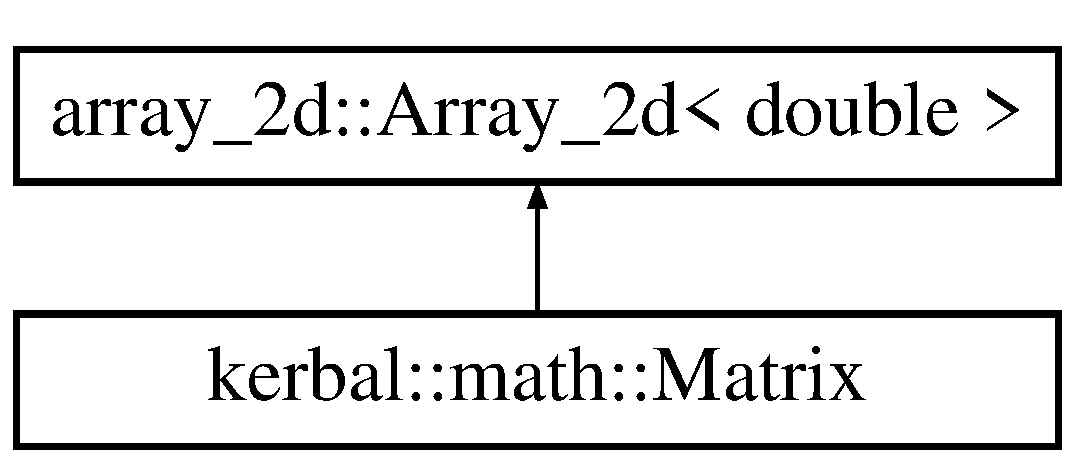
\includegraphics[height=2.000000cm]{classkerbal_1_1math_1_1_matrix}
\end{center}
\end{figure}
\subsection*{Public 类型}
\begin{DoxyCompactItemize}
\item 
enum \hyperlink{classkerbal_1_1math_1_1_matrix_a00dd9ef9c8b8c06f50eed7681f147f71}{Frame} \{ \newline
\hyperlink{classkerbal_1_1math_1_1_matrix_a00dd9ef9c8b8c06f50eed7681f147f71a2ef25fdcf6ef827bf880416bbccb0122}{Fr\+\_\+\+Rt\+Matrix}, 
\hyperlink{classkerbal_1_1math_1_1_matrix_a00dd9ef9c8b8c06f50eed7681f147f71a0589c43464f4819e8208963d92b6c664}{Fr\+\_\+\+Rd\+Matrix}, 
\hyperlink{classkerbal_1_1math_1_1_matrix_a00dd9ef9c8b8c06f50eed7681f147f71aa0277b6e31fe0cf44b854581700e6edb}{Fr\+\_\+\+Det}, 
\hyperlink{classkerbal_1_1math_1_1_matrix_a00dd9ef9c8b8c06f50eed7681f147f71a3b38ac99caab77f29eed02c314db27bf}{Fr\+\_\+double}, 
\newline
\hyperlink{classkerbal_1_1math_1_1_matrix_a00dd9ef9c8b8c06f50eed7681f147f71a57572d7e73fbd562375f1851ba6c31e9}{Fr\+\_\+\+Null}
 \}\begin{DoxyCompactList}\small\item\em 矩阵的输出样式 \end{DoxyCompactList}
\end{DoxyCompactItemize}
\subsection*{Public 成员函数}
\begin{DoxyCompactItemize}
\item 
\mbox{\Hypertarget{classkerbal_1_1math_1_1_matrix_a201ef9e1e51430d7a3cd6ca2093e9981}\label{classkerbal_1_1math_1_1_matrix_a201ef9e1e51430d7a3cd6ca2093e9981}} 
\hyperlink{classkerbal_1_1math_1_1_matrix_a201ef9e1e51430d7a3cd6ca2093e9981}{Matrix} ()  throw ()
\begin{DoxyCompactList}\small\item\em 构造一个 0 行 0 列的空矩阵 \end{DoxyCompactList}\item 
\hyperlink{classkerbal_1_1math_1_1_matrix_a07582c4589d21d351350fce8459c10da}{Matrix} (const int \hyperlink{classarray__2d_1_1_array__2d_a17b90b53a8e0002452e96c2b7f74820b}{row}, const int \hyperlink{classarray__2d_1_1_array__2d_abdf56a1c0f22088353d9a32de9680d76}{column})
\begin{DoxyCompactList}\small\item\em 构造一个 row 行 $\ast$ column 列 的零矩阵 \end{DoxyCompactList}\item 
\hyperlink{classkerbal_1_1math_1_1_matrix_a17111be388a194c33c39946cb7548d79}{Matrix} (const int \hyperlink{classarray__2d_1_1_array__2d_a17b90b53a8e0002452e96c2b7f74820b}{row}, const int \hyperlink{classarray__2d_1_1_array__2d_abdf56a1c0f22088353d9a32de9680d76}{column}, const double \&val)
\begin{DoxyCompactList}\small\item\em 构造一个 row 行 $\ast$ column 列 的矩阵, 矩阵中每个元素的初始值由参数 val 指定 \end{DoxyCompactList}\item 
\mbox{\Hypertarget{classkerbal_1_1math_1_1_matrix_a4cf66d9295ca617254d1fc0d88c33245}\label{classkerbal_1_1math_1_1_matrix_a4cf66d9295ca617254d1fc0d88c33245}} 
{\bfseries Matrix} (double($\ast$function)(), const int \hyperlink{classarray__2d_1_1_array__2d_a17b90b53a8e0002452e96c2b7f74820b}{row}, const int \hyperlink{classarray__2d_1_1_array__2d_abdf56a1c0f22088353d9a32de9680d76}{column}, bool para)
\item 
\mbox{\Hypertarget{classkerbal_1_1math_1_1_matrix_a627aae6f1eb7e9da770730cf75a62c75}\label{classkerbal_1_1math_1_1_matrix_a627aae6f1eb7e9da770730cf75a62c75}} 
{\bfseries Matrix} (double($\ast$function)(int, int), const int \hyperlink{classarray__2d_1_1_array__2d_a17b90b53a8e0002452e96c2b7f74820b}{row}, const int \hyperlink{classarray__2d_1_1_array__2d_abdf56a1c0f22088353d9a32de9680d76}{column}, bool para)
\item 
\mbox{\Hypertarget{classkerbal_1_1math_1_1_matrix_a39f2605c9bd2a647f6f8a7b9dfff804a}\label{classkerbal_1_1math_1_1_matrix_a39f2605c9bd2a647f6f8a7b9dfff804a}} 
{\footnotesize template$<$size\+\_\+t M, size\+\_\+t N$>$ }\\{\bfseries Matrix} (const double(\&src)\mbox{[}M\mbox{]}\mbox{[}N\mbox{]}, const int \hyperlink{classarray__2d_1_1_array__2d_a17b90b53a8e0002452e96c2b7f74820b}{row}, const int \hyperlink{classarray__2d_1_1_array__2d_abdf56a1c0f22088353d9a32de9680d76}{column})
\item 
\mbox{\Hypertarget{classkerbal_1_1math_1_1_matrix_a2b2a8ad8af3e4738dc69a18e5b298577}\label{classkerbal_1_1math_1_1_matrix_a2b2a8ad8af3e4738dc69a18e5b298577}} 
{\bfseries Matrix} (const double arr\mbox{[}$\,$\mbox{]}, int len, bool in\+\_\+a\+\_\+row=true)
\item 
\mbox{\Hypertarget{classkerbal_1_1math_1_1_matrix_aae1f76133d4309d19cf020d413398d19}\label{classkerbal_1_1math_1_1_matrix_aae1f76133d4309d19cf020d413398d19}} 
{\bfseries Matrix} (const \hyperlink{classkerbal_1_1math_1_1_matrix}{Matrix} \&src)
\item 
\mbox{\Hypertarget{classkerbal_1_1math_1_1_matrix_a444d0dcc6f6c0457b8ee3d9c095320ae}\label{classkerbal_1_1math_1_1_matrix_a444d0dcc6f6c0457b8ee3d9c095320ae}} 
virtual \hyperlink{classkerbal_1_1math_1_1_matrix_a444d0dcc6f6c0457b8ee3d9c095320ae}{$\sim$\+Matrix} ()
\begin{DoxyCompactList}\small\item\em 析构函数 \end{DoxyCompactList}\item 
\mbox{\Hypertarget{classkerbal_1_1math_1_1_matrix_a80ea4536d92e0751092997062faaa445}\label{classkerbal_1_1math_1_1_matrix_a80ea4536d92e0751092997062faaa445}} 
virtual void {\bfseries print} (\hyperlink{classkerbal_1_1math_1_1_matrix_a00dd9ef9c8b8c06f50eed7681f147f71}{Frame} frame=\hyperlink{classkerbal_1_1math_1_1_matrix_a00dd9ef9c8b8c06f50eed7681f147f71a2ef25fdcf6ef827bf880416bbccb0122}{Fr\+\_\+\+Rt\+Matrix}, bool print\+\_\+corner=true, std\+::ostream \&output=std\+::cout) const
\item 
\mbox{\Hypertarget{classkerbal_1_1math_1_1_matrix_a0426bb22fd2d5e87b714c03c1a3c8aa4}\label{classkerbal_1_1math_1_1_matrix_a0426bb22fd2d5e87b714c03c1a3c8aa4}} 
void {\bfseries save} (const std\+::string \&file\+\_\+name) const  throw (std\+::runtime\+\_\+error)
\item 
void \hyperlink{classkerbal_1_1math_1_1_matrix_a07d1c06f2a123d7a7366c49c8c884f03}{switch\+\_\+rows} (const int row1, const int row2)  throw (std\+::out\+\_\+of\+\_\+range)
\begin{DoxyCompactList}\small\item\em 交换矩阵的两行 \end{DoxyCompactList}\item 
void \hyperlink{classkerbal_1_1math_1_1_matrix_a47ee8c0afe98e4545233b10f7f7774e8}{switch\+\_\+columns} (const int column1, const int column2)  throw (std\+::out\+\_\+of\+\_\+range)
\begin{DoxyCompactList}\small\item\em 交换矩阵的两列 \end{DoxyCompactList}\item 
void \hyperlink{classkerbal_1_1math_1_1_matrix_add7ad7a55135e85d44437aaceb13ea02}{kmr} (const double k, const int row\+\_\+dest)  throw (std\+::out\+\_\+of\+\_\+range)
\begin{DoxyCompactList}\small\item\em 令矩阵中指定行上的每一个元素均乘上系数 k \end{DoxyCompactList}\item 
void \hyperlink{classkerbal_1_1math_1_1_matrix_aed63e5a9858d007ceaf95efb0f66c221}{kmr\+\_\+plus\+\_\+to\+\_\+another} (const double k, const int row\+\_\+from, const int row\+\_\+dest)  throw (std\+::out\+\_\+of\+\_\+range)
\begin{DoxyCompactList}\small\item\em 将矩阵 row\+\_\+from 行的 k 倍加到 row\+\_\+dest 行上 \end{DoxyCompactList}\item 
void \hyperlink{classkerbal_1_1math_1_1_matrix_aed36c6097e228052c76e437a4cb195b7}{kmc} (const double k, const int column\+\_\+dest)  throw (std\+::out\+\_\+of\+\_\+range)
\begin{DoxyCompactList}\small\item\em 令矩阵中指定列上的每一个元素均乘上系数 k \end{DoxyCompactList}\item 
\mbox{\Hypertarget{classkerbal_1_1math_1_1_matrix_aa7cc2a11d47aa71b7609c4e92cb86b1c}\label{classkerbal_1_1math_1_1_matrix_aa7cc2a11d47aa71b7609c4e92cb86b1c}} 
void {\bfseries kmc\+\_\+plus\+\_\+to\+\_\+another} (const double k, const int column\+\_\+from, const int column\+\_\+dest)  throw (std\+::out\+\_\+of\+\_\+range)
\item 
\mbox{\Hypertarget{classkerbal_1_1math_1_1_matrix_abceaa9468b6280a4d3dfd6fe34141ac1}\label{classkerbal_1_1math_1_1_matrix_abceaa9468b6280a4d3dfd6fe34141ac1}} 
void {\bfseries do\+\_\+optimize\+\_\+rows} ()  throw (std\+::invalid\+\_\+argument)
\item 
\mbox{\Hypertarget{classkerbal_1_1math_1_1_matrix_a7289f2b36f95af690b62f11131854cf3}\label{classkerbal_1_1math_1_1_matrix_a7289f2b36f95af690b62f11131854cf3}} 
double {\bfseries det} () const  throw (std\+::invalid\+\_\+argument)
\item 
\mbox{\Hypertarget{classkerbal_1_1math_1_1_matrix_af05f82ae450547615242aa9249f48eb8}\label{classkerbal_1_1math_1_1_matrix_af05f82ae450547615242aa9249f48eb8}} 
\hyperlink{classkerbal_1_1math_1_1_matrix}{Matrix} {\bfseries Adjugate\+\_\+matrix} () const  throw (std\+::invalid\+\_\+argument)
\item 
\mbox{\Hypertarget{classkerbal_1_1math_1_1_matrix_a261f7c5a383008954f0b806f8b25b152}\label{classkerbal_1_1math_1_1_matrix_a261f7c5a383008954f0b806f8b25b152}} 
\hyperlink{classkerbal_1_1math_1_1_matrix}{Matrix} {\bfseries Inverse\+\_\+matrix} () const  throw (std\+::invalid\+\_\+argument)
\item 
\mbox{\Hypertarget{classkerbal_1_1math_1_1_matrix_aa074455d62b7f76562b58626997e70df}\label{classkerbal_1_1math_1_1_matrix_aa074455d62b7f76562b58626997e70df}} 
const \hyperlink{classkerbal_1_1math_1_1_matrix}{Matrix} {\bfseries operator+} () const
\item 
\mbox{\Hypertarget{classkerbal_1_1math_1_1_matrix_a0b2c1bd12d1064bebc2fa195f5c680d2}\label{classkerbal_1_1math_1_1_matrix_a0b2c1bd12d1064bebc2fa195f5c680d2}} 
const \hyperlink{classkerbal_1_1math_1_1_matrix}{Matrix} {\bfseries operator-\/} () const
\item 
\hyperlink{classkerbal_1_1math_1_1_matrix}{Matrix} \& \hyperlink{classkerbal_1_1math_1_1_matrix_a2adadd6868dbd09192a77655dc54a580}{operator+=} (const \hyperlink{classkerbal_1_1math_1_1_matrix}{Matrix} \&with)  throw (std\+::invalid\+\_\+argument)
\begin{DoxyCompactList}\small\item\em 令赋值运算符前的矩阵加上赋值运算符后的矩阵 \end{DoxyCompactList}\item 
\hyperlink{classkerbal_1_1math_1_1_matrix}{Matrix} \& \hyperlink{classkerbal_1_1math_1_1_matrix_a4fcc469526f1c13aab912278ba69dd85}{operator-\/=} (const \hyperlink{classkerbal_1_1math_1_1_matrix}{Matrix} \&with)  throw (std\+::invalid\+\_\+argument)
\begin{DoxyCompactList}\small\item\em 令赋值运算符前的矩阵减去赋值运算符后的矩阵 \end{DoxyCompactList}\item 
\hyperlink{classkerbal_1_1math_1_1_matrix}{Matrix} \& \hyperlink{classkerbal_1_1math_1_1_matrix_a37786e33296ebea6c97d12d1e659a693}{operator$\ast$=} (double k)  throw ()
\begin{DoxyCompactList}\small\item\em 令一个矩阵的每一个元素均乘以系数 k \end{DoxyCompactList}\item 
\mbox{\Hypertarget{classkerbal_1_1math_1_1_matrix_ac29bf818dcb33bc853ce585fff476943}\label{classkerbal_1_1math_1_1_matrix_ac29bf818dcb33bc853ce585fff476943}} 
\hyperlink{classkerbal_1_1math_1_1_matrix}{Matrix} \& {\bfseries operator=} (const \hyperlink{classkerbal_1_1math_1_1_matrix}{Matrix} \&src)
\item 
\mbox{\Hypertarget{classkerbal_1_1math_1_1_matrix_aba372953226341b1d4492d569e02cb97}\label{classkerbal_1_1math_1_1_matrix_aba372953226341b1d4492d569e02cb97}} 
const \hyperlink{classkerbal_1_1math_1_1_matrix}{Matrix} {\bfseries sub\+\_\+of} (int up, int down, int left, int right) const  throw (std\+::invalid\+\_\+argument, std\+::out\+\_\+of\+\_\+range)
\item 
\mbox{\Hypertarget{classkerbal_1_1math_1_1_matrix_a95cba7989eb6db03ffc3062b77380649}\label{classkerbal_1_1math_1_1_matrix_a95cba7989eb6db03ffc3062b77380649}} 
void {\bfseries do\+\_\+transpose} ()
\item 
\mbox{\Hypertarget{classkerbal_1_1math_1_1_matrix_a8c694cdf011ad8cae04c20b55ae24026}\label{classkerbal_1_1math_1_1_matrix_a8c694cdf011ad8cae04c20b55ae24026}} 
void {\bfseries do\+\_\+cofactor} (const int row\+\_\+tar, const int column\+\_\+tar)  throw (std\+::out\+\_\+of\+\_\+range)
\item 
\mbox{\Hypertarget{classkerbal_1_1math_1_1_matrix_a06ed57fda8ee54bd37a22aa9acdb1497}\label{classkerbal_1_1math_1_1_matrix_a06ed57fda8ee54bd37a22aa9acdb1497}} 
virtual void {\bfseries test\+\_\+row} (const int row\+\_\+test) const  throw (std\+::out\+\_\+of\+\_\+range)
\item 
\mbox{\Hypertarget{classkerbal_1_1math_1_1_matrix_a3e7f26fdef23c5e0e6bb60aea37db72f}\label{classkerbal_1_1math_1_1_matrix_a3e7f26fdef23c5e0e6bb60aea37db72f}} 
virtual void {\bfseries test\+\_\+column} (const int column\+\_\+test) const  throw (std\+::out\+\_\+of\+\_\+range)
\item 
\mbox{\Hypertarget{classkerbal_1_1math_1_1_matrix_ae7a03096165bb72e4c361476f02b2d23}\label{classkerbal_1_1math_1_1_matrix_ae7a03096165bb72e4c361476f02b2d23}} 
void {\bfseries test\+\_\+square} () const  throw (std\+::invalid\+\_\+argument)
\end{DoxyCompactItemize}
\subsection*{静态 Public 成员函数}
\begin{DoxyCompactItemize}
\item 
\mbox{\Hypertarget{classkerbal_1_1math_1_1_matrix_a19d3d26c63d7598205a6d064b68a6bd4}\label{classkerbal_1_1math_1_1_matrix_a19d3d26c63d7598205a6d064b68a6bd4}} 
static const \hyperlink{classkerbal_1_1math_1_1_matrix}{Matrix} {\bfseries load\+\_\+from} (const std\+::string \&file\+\_\+name)
\end{DoxyCompactItemize}
\subsection*{友元}
\begin{DoxyCompactItemize}
\item 
const \hyperlink{classkerbal_1_1math_1_1_matrix}{Matrix} \hyperlink{classkerbal_1_1math_1_1_matrix_a68ca5b1d7d0aaf615a63771788562210}{operator+} (const \hyperlink{classkerbal_1_1math_1_1_matrix}{Matrix} \&A, const \hyperlink{classkerbal_1_1math_1_1_matrix}{Matrix} \&B)  throw (std\+::invalid\+\_\+argument)
\begin{DoxyCompactList}\small\item\em 计算两个矩阵的加法 \end{DoxyCompactList}\item 
const \hyperlink{classkerbal_1_1math_1_1_matrix}{Matrix} \hyperlink{classkerbal_1_1math_1_1_matrix_a4fc480fab44a4d6c69a6cf92f91522ad}{operator-\/} (const \hyperlink{classkerbal_1_1math_1_1_matrix}{Matrix} \&A, const \hyperlink{classkerbal_1_1math_1_1_matrix}{Matrix} \&B)  throw (std\+::invalid\+\_\+argument)
\begin{DoxyCompactList}\small\item\em 计算两个矩阵的减法 \end{DoxyCompactList}\item 
\mbox{\Hypertarget{classkerbal_1_1math_1_1_matrix_ae4dae004adfcec267b060864b1fcfa41}\label{classkerbal_1_1math_1_1_matrix_ae4dae004adfcec267b060864b1fcfa41}} 
const \hyperlink{classkerbal_1_1math_1_1_matrix}{Matrix} {\bfseries operator$\ast$} (const double k, const \hyperlink{classkerbal_1_1math_1_1_matrix}{Matrix} \&A)  throw ()
\item 
\mbox{\Hypertarget{classkerbal_1_1math_1_1_matrix_a2c961c7157712ed49125788e6bee2e23}\label{classkerbal_1_1math_1_1_matrix_a2c961c7157712ed49125788e6bee2e23}} 
const \hyperlink{classkerbal_1_1math_1_1_matrix}{Matrix} {\bfseries operator$\ast$} (const \hyperlink{classkerbal_1_1math_1_1_matrix}{Matrix} \&A, const double k)  throw ()
\item 
\mbox{\Hypertarget{classkerbal_1_1math_1_1_matrix_a26be23966c1457aaa6ca7904f3388504}\label{classkerbal_1_1math_1_1_matrix_a26be23966c1457aaa6ca7904f3388504}} 
const \hyperlink{classkerbal_1_1math_1_1_matrix}{Matrix} {\bfseries operator$\ast$} (const \hyperlink{classkerbal_1_1math_1_1_matrix}{Matrix} \&A, const \hyperlink{classkerbal_1_1math_1_1_matrix}{Matrix} \&B)  throw (std\+::invalid\+\_\+argument)
\item 
const \hyperlink{classkerbal_1_1math_1_1_matrix}{Matrix} \hyperlink{classkerbal_1_1math_1_1_matrix_aef00278756b7155aa065aa0e2c206b91}{fma} (const \hyperlink{classkerbal_1_1math_1_1_matrix}{Matrix} \&A, const \hyperlink{classkerbal_1_1math_1_1_matrix}{Matrix} \&B, const \hyperlink{classkerbal_1_1math_1_1_matrix}{Matrix} \&C)  throw (std\+::invalid\+\_\+argument)
\begin{DoxyCompactList}\small\item\em 计算 (A $\ast$ B) + C 的结果 \end{DoxyCompactList}\item 
const \hyperlink{classkerbal_1_1math_1_1_matrix}{Matrix} \hyperlink{classkerbal_1_1math_1_1_matrix_a34aab263e821d766d31517e9d03a1aca}{dot\+\_\+product} (const \hyperlink{classkerbal_1_1math_1_1_matrix}{Matrix} \&A, const \hyperlink{classkerbal_1_1math_1_1_matrix}{Matrix} \&B)  throw (std\+::invalid\+\_\+argument)
\begin{DoxyCompactList}\small\item\em 计算两个矩阵的点乘 \end{DoxyCompactList}\item 
const \hyperlink{classkerbal_1_1math_1_1_matrix}{Matrix} \hyperlink{classkerbal_1_1math_1_1_matrix_af46d90e12227e9e1e8c8242cb2b0a93a}{operator$^\wedge$} (const \hyperlink{classkerbal_1_1math_1_1_matrix}{Matrix} \&A, const int n)  throw (std\+::invalid\+\_\+argument)
\begin{DoxyCompactList}\small\item\em 计算一个矩阵的 n 次幂 \end{DoxyCompactList}\item 
const \hyperlink{classkerbal_1_1math_1_1_matrix}{Matrix} \hyperlink{classkerbal_1_1math_1_1_matrix_a8b58a45223c7264d0e45d238f66b1eb5}{operator \&\&} (const \hyperlink{classkerbal_1_1math_1_1_matrix}{Matrix} \&A, const \hyperlink{classkerbal_1_1math_1_1_matrix}{Matrix} \&B)  throw (std\+::invalid\+\_\+argument)
\begin{DoxyCompactList}\small\item\em 将两个矩阵按竖直方向连接 \end{DoxyCompactList}\item 
const \hyperlink{classkerbal_1_1math_1_1_matrix}{Matrix} \hyperlink{classkerbal_1_1math_1_1_matrix_aaa58ea23f11a2f1ad42b487f9a6d0245}{operator$\vert$$\vert$} (const \hyperlink{classkerbal_1_1math_1_1_matrix}{Matrix} \&A, const \hyperlink{classkerbal_1_1math_1_1_matrix}{Matrix} \&B)  throw (std\+::invalid\+\_\+argument)
\begin{DoxyCompactList}\small\item\em 将两个矩阵按水平方向连接 \end{DoxyCompactList}\item 
\mbox{\Hypertarget{classkerbal_1_1math_1_1_matrix_ad6baacfd0e9f61f34af177147b55939a}\label{classkerbal_1_1math_1_1_matrix_ad6baacfd0e9f61f34af177147b55939a}} 
void {\bfseries operator$<$$<$=} (\hyperlink{classkerbal_1_1math_1_1_matrix}{Matrix} \&tar, \hyperlink{classkerbal_1_1math_1_1_matrix}{Matrix} \&src)
\item 
\mbox{\Hypertarget{classkerbal_1_1math_1_1_matrix_a8b595740f508d34b7cff5e159b44bcc0}\label{classkerbal_1_1math_1_1_matrix_a8b595740f508d34b7cff5e159b44bcc0}} 
{\footnotesize template$<$size\+\_\+t N$>$ }\\const \hyperlink{classkerbal_1_1math_1_1_matrix}{Matrix} {\bfseries cat} (const \hyperlink{classkerbal_1_1math_1_1_matrix}{Matrix}(\&a)\mbox{[}N\mbox{]})  throw (std\+::invalid\+\_\+argument)
\item 
const \hyperlink{classkerbal_1_1math_1_1_matrix}{Matrix} \hyperlink{classkerbal_1_1math_1_1_matrix_a66d6a7eb6b57a6e5acb75ab8b4349471}{eye} (int n)
\begin{DoxyCompactList}\small\item\em 返回一个 n 阶单位矩阵 \end{DoxyCompactList}\item 
const \hyperlink{classkerbal_1_1math_1_1_matrix}{Matrix} \hyperlink{classkerbal_1_1math_1_1_matrix_a35bd334cc41142e574a3261853fd14d2}{pow} (const \hyperlink{classkerbal_1_1math_1_1_matrix}{Matrix} \&A, const int n)  throw (std\+::invalid\+\_\+argument)
\begin{DoxyCompactList}\small\item\em 计算一个矩阵的 n 次幂 \end{DoxyCompactList}\item 
\mbox{\Hypertarget{classkerbal_1_1math_1_1_matrix_ab5a14c5b61c616fa699113c704c046c4}\label{classkerbal_1_1math_1_1_matrix_ab5a14c5b61c616fa699113c704c046c4}} 
double {\bfseries tr} (const \hyperlink{classkerbal_1_1math_1_1_matrix}{Matrix} \&src)  throw (std\+::invalid\+\_\+argument)
\item 
\mbox{\Hypertarget{classkerbal_1_1math_1_1_matrix_aca59235f2426e023a982b2424c116a12}\label{classkerbal_1_1math_1_1_matrix_aca59235f2426e023a982b2424c116a12}} 
const \hyperlink{classkerbal_1_1math_1_1_matrix}{Matrix} {\bfseries transpose\+\_\+of} (const \hyperlink{classkerbal_1_1math_1_1_matrix}{Matrix} \&A)
\item 
\mbox{\Hypertarget{classkerbal_1_1math_1_1_matrix_a0e0f686216ed93f7a1c962006a0c7ff1}\label{classkerbal_1_1math_1_1_matrix_a0e0f686216ed93f7a1c962006a0c7ff1}} 
const \hyperlink{classkerbal_1_1math_1_1_matrix}{Matrix} {\bfseries cofactor\+\_\+of} (const \hyperlink{classkerbal_1_1math_1_1_matrix}{Matrix} \&A, const int x, const int y)  throw (std\+::out\+\_\+of\+\_\+range)
\item 
\mbox{\Hypertarget{classkerbal_1_1math_1_1_matrix_a17b7efc841868072cabb906fb2ee0a3a}\label{classkerbal_1_1math_1_1_matrix_a17b7efc841868072cabb906fb2ee0a3a}} 
bool {\bfseries Matcmp} (const \hyperlink{classkerbal_1_1math_1_1_matrix}{Matrix} \&A, const \hyperlink{classkerbal_1_1math_1_1_matrix}{Matrix} \&B, double eps)
\item 
\mbox{\Hypertarget{classkerbal_1_1math_1_1_matrix_a6f53d61daeba794daa792db83f92a8e2}\label{classkerbal_1_1math_1_1_matrix_a6f53d61daeba794daa792db83f92a8e2}} 
const \hyperlink{classkerbal_1_1math_1_1_matrix}{Matrix} {\bfseries conv2} (const \hyperlink{classkerbal_1_1math_1_1_matrix}{Matrix} \&core, const \hyperlink{classkerbal_1_1math_1_1_matrix}{Matrix} \&B, int size=0)
\item 
\mbox{\Hypertarget{classkerbal_1_1math_1_1_matrix_a13d83eac9b443b09ea698e9e9d0b3848}\label{classkerbal_1_1math_1_1_matrix_a13d83eac9b443b09ea698e9e9d0b3848}} 
void {\bfseries std\+::swap} (\hyperlink{classkerbal_1_1math_1_1_matrix}{Matrix} \&a, \hyperlink{classkerbal_1_1math_1_1_matrix}{Matrix} \&b)
\end{DoxyCompactItemize}
\subsection*{额外继承的成员函数}


\subsection{详细描述}
矩阵类 

\begin{DoxyAuthor}{作者}
倪文卿 
\end{DoxyAuthor}


\subsection{成员枚举类型说明}
\mbox{\Hypertarget{classkerbal_1_1math_1_1_matrix_a00dd9ef9c8b8c06f50eed7681f147f71}\label{classkerbal_1_1math_1_1_matrix_a00dd9ef9c8b8c06f50eed7681f147f71}} 
\index{kerbal\+::math\+::\+Matrix@{kerbal\+::math\+::\+Matrix}!Frame@{Frame}}
\index{Frame@{Frame}!kerbal\+::math\+::\+Matrix@{kerbal\+::math\+::\+Matrix}}
\subsubsection{\texorpdfstring{Frame}{Frame}}
{\footnotesize\ttfamily enum \hyperlink{classkerbal_1_1math_1_1_matrix_a00dd9ef9c8b8c06f50eed7681f147f71}{kerbal\+::math\+::\+Matrix\+::\+Frame}}



矩阵的输出样式 

\begin{DoxyEnumFields}{枚举值}
\raisebox{\heightof{T}}[0pt][0pt]{\index{Fr\+\_\+\+Rt\+Matrix@{Fr\+\_\+\+Rt\+Matrix}!kerbal\+::math\+::\+Matrix@{kerbal\+::math\+::\+Matrix}}\index{kerbal\+::math\+::\+Matrix@{kerbal\+::math\+::\+Matrix}!Fr\+\_\+\+Rt\+Matrix@{Fr\+\_\+\+Rt\+Matrix}}}\mbox{\Hypertarget{classkerbal_1_1math_1_1_matrix_a00dd9ef9c8b8c06f50eed7681f147f71a2ef25fdcf6ef827bf880416bbccb0122}\label{classkerbal_1_1math_1_1_matrix_a00dd9ef9c8b8c06f50eed7681f147f71a2ef25fdcf6ef827bf880416bbccb0122}} 
Fr\+\_\+\+Rt\+Matrix&输出直角 Fr\+\_\+\+Rt\+Matrix \\
\hline

\raisebox{\heightof{T}}[0pt][0pt]{\index{Fr\+\_\+\+Rd\+Matrix@{Fr\+\_\+\+Rd\+Matrix}!kerbal\+::math\+::\+Matrix@{kerbal\+::math\+::\+Matrix}}\index{kerbal\+::math\+::\+Matrix@{kerbal\+::math\+::\+Matrix}!Fr\+\_\+\+Rd\+Matrix@{Fr\+\_\+\+Rd\+Matrix}}}\mbox{\Hypertarget{classkerbal_1_1math_1_1_matrix_a00dd9ef9c8b8c06f50eed7681f147f71a0589c43464f4819e8208963d92b6c664}\label{classkerbal_1_1math_1_1_matrix_a00dd9ef9c8b8c06f50eed7681f147f71a0589c43464f4819e8208963d92b6c664}} 
Fr\+\_\+\+Rd\+Matrix&输出圆角 Fr\+\_\+\+Rd\+Matrix \\
\hline

\raisebox{\heightof{T}}[0pt][0pt]{\index{Fr\+\_\+\+Det@{Fr\+\_\+\+Det}!kerbal\+::math\+::\+Matrix@{kerbal\+::math\+::\+Matrix}}\index{kerbal\+::math\+::\+Matrix@{kerbal\+::math\+::\+Matrix}!Fr\+\_\+\+Det@{Fr\+\_\+\+Det}}}\mbox{\Hypertarget{classkerbal_1_1math_1_1_matrix_a00dd9ef9c8b8c06f50eed7681f147f71aa0277b6e31fe0cf44b854581700e6edb}\label{classkerbal_1_1math_1_1_matrix_a00dd9ef9c8b8c06f50eed7681f147f71aa0277b6e31fe0cf44b854581700e6edb}} 
Fr\+\_\+\+Det&输出行列式 Fr\+\_\+\+Det \\
\hline

\raisebox{\heightof{T}}[0pt][0pt]{\index{Fr\+\_\+double@{Fr\+\_\+double}!kerbal\+::math\+::\+Matrix@{kerbal\+::math\+::\+Matrix}}\index{kerbal\+::math\+::\+Matrix@{kerbal\+::math\+::\+Matrix}!Fr\+\_\+double@{Fr\+\_\+double}}}\mbox{\Hypertarget{classkerbal_1_1math_1_1_matrix_a00dd9ef9c8b8c06f50eed7681f147f71a3b38ac99caab77f29eed02c314db27bf}\label{classkerbal_1_1math_1_1_matrix_a00dd9ef9c8b8c06f50eed7681f147f71a3b38ac99caab77f29eed02c314db27bf}} 
Fr\+\_\+double&输出双竖线 Fr\+\_\+double \\
\hline

\raisebox{\heightof{T}}[0pt][0pt]{\index{Fr\+\_\+\+Null@{Fr\+\_\+\+Null}!kerbal\+::math\+::\+Matrix@{kerbal\+::math\+::\+Matrix}}\index{kerbal\+::math\+::\+Matrix@{kerbal\+::math\+::\+Matrix}!Fr\+\_\+\+Null@{Fr\+\_\+\+Null}}}\mbox{\Hypertarget{classkerbal_1_1math_1_1_matrix_a00dd9ef9c8b8c06f50eed7681f147f71a57572d7e73fbd562375f1851ba6c31e9}\label{classkerbal_1_1math_1_1_matrix_a00dd9ef9c8b8c06f50eed7681f147f71a57572d7e73fbd562375f1851ba6c31e9}} 
Fr\+\_\+\+Null&无边框 Fr\+\_\+\+Null \\
\hline

\end{DoxyEnumFields}


\subsection{构造及析构函数说明}
\mbox{\Hypertarget{classkerbal_1_1math_1_1_matrix_a07582c4589d21d351350fce8459c10da}\label{classkerbal_1_1math_1_1_matrix_a07582c4589d21d351350fce8459c10da}} 
\index{kerbal\+::math\+::\+Matrix@{kerbal\+::math\+::\+Matrix}!Matrix@{Matrix}}
\index{Matrix@{Matrix}!kerbal\+::math\+::\+Matrix@{kerbal\+::math\+::\+Matrix}}
\subsubsection{\texorpdfstring{Matrix()}{Matrix()}\hspace{0.1cm}{\footnotesize\ttfamily [1/2]}}
{\footnotesize\ttfamily kerbal\+::math\+::\+Matrix\+::\+Matrix (\begin{DoxyParamCaption}\item[{const int}]{row,  }\item[{const int}]{column }\end{DoxyParamCaption})}



构造一个 row 行 $\ast$ column 列 的零矩阵 


\begin{DoxyParams}{参数}
{\em row} & 行数 \\
\hline
{\em column} & 列数 \\
\hline
\end{DoxyParams}
\mbox{\Hypertarget{classkerbal_1_1math_1_1_matrix_a17111be388a194c33c39946cb7548d79}\label{classkerbal_1_1math_1_1_matrix_a17111be388a194c33c39946cb7548d79}} 
\index{kerbal\+::math\+::\+Matrix@{kerbal\+::math\+::\+Matrix}!Matrix@{Matrix}}
\index{Matrix@{Matrix}!kerbal\+::math\+::\+Matrix@{kerbal\+::math\+::\+Matrix}}
\subsubsection{\texorpdfstring{Matrix()}{Matrix()}\hspace{0.1cm}{\footnotesize\ttfamily [2/2]}}
{\footnotesize\ttfamily kerbal\+::math\+::\+Matrix\+::\+Matrix (\begin{DoxyParamCaption}\item[{const int}]{row,  }\item[{const int}]{column,  }\item[{const double \&}]{val }\end{DoxyParamCaption})}



构造一个 row 行 $\ast$ column 列 的矩阵, 矩阵中每个元素的初始值由参数 val 指定 


\begin{DoxyParams}{参数}
{\em row} & 行数 \\
\hline
{\em column} & 列数 \\
\hline
{\em val} & 初始值 \\
\hline
\end{DoxyParams}


\subsection{成员函数说明}
\mbox{\Hypertarget{classkerbal_1_1math_1_1_matrix_aed36c6097e228052c76e437a4cb195b7}\label{classkerbal_1_1math_1_1_matrix_aed36c6097e228052c76e437a4cb195b7}} 
\index{kerbal\+::math\+::\+Matrix@{kerbal\+::math\+::\+Matrix}!kmc@{kmc}}
\index{kmc@{kmc}!kerbal\+::math\+::\+Matrix@{kerbal\+::math\+::\+Matrix}}
\subsubsection{\texorpdfstring{kmc()}{kmc()}}
{\footnotesize\ttfamily void kerbal\+::math\+::\+Matrix\+::kmc (\begin{DoxyParamCaption}\item[{const double}]{k,  }\item[{const int}]{column\+\_\+dest }\end{DoxyParamCaption}) throw  std\+::out\+\_\+of\+\_\+range) }



令矩阵中指定列上的每一个元素均乘上系数 k 


\begin{DoxyParams}{参数}
{\em k} & 系数 \\
\hline
{\em column\+\_\+dest} & 被乘列列号 \\
\hline
\end{DoxyParams}
\mbox{\Hypertarget{classkerbal_1_1math_1_1_matrix_add7ad7a55135e85d44437aaceb13ea02}\label{classkerbal_1_1math_1_1_matrix_add7ad7a55135e85d44437aaceb13ea02}} 
\index{kerbal\+::math\+::\+Matrix@{kerbal\+::math\+::\+Matrix}!kmr@{kmr}}
\index{kmr@{kmr}!kerbal\+::math\+::\+Matrix@{kerbal\+::math\+::\+Matrix}}
\subsubsection{\texorpdfstring{kmr()}{kmr()}}
{\footnotesize\ttfamily void kerbal\+::math\+::\+Matrix\+::kmr (\begin{DoxyParamCaption}\item[{const double}]{k,  }\item[{const int}]{row\+\_\+dest }\end{DoxyParamCaption}) throw  std\+::out\+\_\+of\+\_\+range) }



令矩阵中指定行上的每一个元素均乘上系数 k 


\begin{DoxyParams}{参数}
{\em k} & 系数 \\
\hline
{\em row\+\_\+dest} & 被乘行行号 \\
\hline
\end{DoxyParams}

\begin{DoxyExceptions}{异常}
{\em std\+::out\+\_\+of\+\_\+range} & 若参数 row\+\_\+dest 越界, 则抛出此异常 \\
\hline
\end{DoxyExceptions}
\mbox{\Hypertarget{classkerbal_1_1math_1_1_matrix_aed63e5a9858d007ceaf95efb0f66c221}\label{classkerbal_1_1math_1_1_matrix_aed63e5a9858d007ceaf95efb0f66c221}} 
\index{kerbal\+::math\+::\+Matrix@{kerbal\+::math\+::\+Matrix}!kmr\+\_\+plus\+\_\+to\+\_\+another@{kmr\+\_\+plus\+\_\+to\+\_\+another}}
\index{kmr\+\_\+plus\+\_\+to\+\_\+another@{kmr\+\_\+plus\+\_\+to\+\_\+another}!kerbal\+::math\+::\+Matrix@{kerbal\+::math\+::\+Matrix}}
\subsubsection{\texorpdfstring{kmr\+\_\+plus\+\_\+to\+\_\+another()}{kmr\_plus\_to\_another()}}
{\footnotesize\ttfamily void kerbal\+::math\+::\+Matrix\+::kmr\+\_\+plus\+\_\+to\+\_\+another (\begin{DoxyParamCaption}\item[{const double}]{k,  }\item[{const int}]{row\+\_\+from,  }\item[{const int}]{row\+\_\+dest }\end{DoxyParamCaption}) throw  std\+::out\+\_\+of\+\_\+range) }



将矩阵 row\+\_\+from 行的 k 倍加到 row\+\_\+dest 行上 


\begin{DoxyParams}{参数}
{\em k} & 系数 \\
\hline
{\em row\+\_\+from} & 被乘行行号 \\
\hline
{\em row\+\_\+dest} & 被加行行号 \\
\hline
\end{DoxyParams}

\begin{DoxyExceptions}{异常}
{\em std\+::out\+\_\+of\+\_\+range} & 若参数 row\+\_\+from 或 row\+\_\+dest 越界, 则抛出此异常 \\
\hline
\end{DoxyExceptions}
\mbox{\Hypertarget{classkerbal_1_1math_1_1_matrix_a37786e33296ebea6c97d12d1e659a693}\label{classkerbal_1_1math_1_1_matrix_a37786e33296ebea6c97d12d1e659a693}} 
\index{kerbal\+::math\+::\+Matrix@{kerbal\+::math\+::\+Matrix}!operator$\ast$=@{operator$\ast$=}}
\index{operator$\ast$=@{operator$\ast$=}!kerbal\+::math\+::\+Matrix@{kerbal\+::math\+::\+Matrix}}
\subsubsection{\texorpdfstring{operator$\ast$=()}{operator*=()}}
{\footnotesize\ttfamily \hyperlink{classkerbal_1_1math_1_1_matrix}{Matrix} \& kerbal\+::math\+::\+Matrix\+::operator$\ast$= (\begin{DoxyParamCaption}\item[{double}]{k }\end{DoxyParamCaption}) throw  ) }



令一个矩阵的每一个元素均乘以系数 k 


\begin{DoxyParams}{参数}
{\em k} & 系数 k \\
\hline
\end{DoxyParams}
\begin{DoxyReturn}{返回}
赋值运算符前被乘矩阵的引用 
\end{DoxyReturn}

\begin{DoxyExceptions}{异常}
{\em 此方法保证不抛出任何异常} & \\
\hline
\end{DoxyExceptions}
\begin{DoxyRemark}{备注}
此方法等效于 m = m $\ast$ k 或 m = k $\ast$ m , 不过具有更佳的效率 
\end{DoxyRemark}
\mbox{\Hypertarget{classkerbal_1_1math_1_1_matrix_a2adadd6868dbd09192a77655dc54a580}\label{classkerbal_1_1math_1_1_matrix_a2adadd6868dbd09192a77655dc54a580}} 
\index{kerbal\+::math\+::\+Matrix@{kerbal\+::math\+::\+Matrix}!operator+=@{operator+=}}
\index{operator+=@{operator+=}!kerbal\+::math\+::\+Matrix@{kerbal\+::math\+::\+Matrix}}
\subsubsection{\texorpdfstring{operator+=()}{operator+=()}}
{\footnotesize\ttfamily \hyperlink{classkerbal_1_1math_1_1_matrix}{Matrix} \& kerbal\+::math\+::\+Matrix\+::operator+= (\begin{DoxyParamCaption}\item[{const \hyperlink{classkerbal_1_1math_1_1_matrix}{Matrix} \&}]{with }\end{DoxyParamCaption}) throw  std\+::invalid\+\_\+argument) }



令赋值运算符前的矩阵加上赋值运算符后的矩阵 


\begin{DoxyParams}{参数}
{\em with} & 加上的矩阵 \\
\hline
\end{DoxyParams}
\begin{DoxyReturn}{返回}
赋值运算符前被加矩阵的引用 
\end{DoxyReturn}

\begin{DoxyExceptions}{异常}
{\em std\+::invalid\+\_\+argument} & 当两个矩阵大小不一致时, 抛出此异常 \\
\hline
\end{DoxyExceptions}
\begin{DoxyRemark}{备注}
此方法等效于 m = m + with 或 m = with + m , 不过具有更佳的效率 
\end{DoxyRemark}
\mbox{\Hypertarget{classkerbal_1_1math_1_1_matrix_a4fcc469526f1c13aab912278ba69dd85}\label{classkerbal_1_1math_1_1_matrix_a4fcc469526f1c13aab912278ba69dd85}} 
\index{kerbal\+::math\+::\+Matrix@{kerbal\+::math\+::\+Matrix}!operator-\/=@{operator-\/=}}
\index{operator-\/=@{operator-\/=}!kerbal\+::math\+::\+Matrix@{kerbal\+::math\+::\+Matrix}}
\subsubsection{\texorpdfstring{operator-\/=()}{operator-=()}}
{\footnotesize\ttfamily \hyperlink{classkerbal_1_1math_1_1_matrix}{Matrix} \& kerbal\+::math\+::\+Matrix\+::operator-\/= (\begin{DoxyParamCaption}\item[{const \hyperlink{classkerbal_1_1math_1_1_matrix}{Matrix} \&}]{with }\end{DoxyParamCaption}) throw  std\+::invalid\+\_\+argument) }



令赋值运算符前的矩阵减去赋值运算符后的矩阵 


\begin{DoxyParams}{参数}
{\em with} & 减去的矩阵 \\
\hline
\end{DoxyParams}
\begin{DoxyReturn}{返回}
赋值运算符前被减矩阵的引用 
\end{DoxyReturn}

\begin{DoxyExceptions}{异常}
{\em std\+::invalid\+\_\+argument} & 当两个矩阵大小不一致时, 抛出此异常 \\
\hline
\end{DoxyExceptions}
\begin{DoxyRemark}{备注}
此方法等效于 m = m -\/ with , 不过具有更佳的效率 
\end{DoxyRemark}
\mbox{\Hypertarget{classkerbal_1_1math_1_1_matrix_a47ee8c0afe98e4545233b10f7f7774e8}\label{classkerbal_1_1math_1_1_matrix_a47ee8c0afe98e4545233b10f7f7774e8}} 
\index{kerbal\+::math\+::\+Matrix@{kerbal\+::math\+::\+Matrix}!switch\+\_\+columns@{switch\+\_\+columns}}
\index{switch\+\_\+columns@{switch\+\_\+columns}!kerbal\+::math\+::\+Matrix@{kerbal\+::math\+::\+Matrix}}
\subsubsection{\texorpdfstring{switch\+\_\+columns()}{switch\_columns()}}
{\footnotesize\ttfamily void kerbal\+::math\+::\+Matrix\+::switch\+\_\+columns (\begin{DoxyParamCaption}\item[{const int}]{column1,  }\item[{const int}]{column2 }\end{DoxyParamCaption}) throw  std\+::out\+\_\+of\+\_\+range) }



交换矩阵的两列 


\begin{DoxyParams}{参数}
{\em column1} & 列号1 \\
\hline
{\em column2} & 列号2 \\
\hline
\end{DoxyParams}

\begin{DoxyExceptions}{异常}
{\em std\+::out\+\_\+of\+\_\+range} & 若参数 column1 或 column2 越界, 则抛出此异常 \\
\hline
\end{DoxyExceptions}
\begin{DoxyParagraph}{时间复杂度}
此操作具有 O(row) 阶复杂度. 其中, row 表示被操作矩阵的行数 
\end{DoxyParagraph}
\mbox{\Hypertarget{classkerbal_1_1math_1_1_matrix_a07d1c06f2a123d7a7366c49c8c884f03}\label{classkerbal_1_1math_1_1_matrix_a07d1c06f2a123d7a7366c49c8c884f03}} 
\index{kerbal\+::math\+::\+Matrix@{kerbal\+::math\+::\+Matrix}!switch\+\_\+rows@{switch\+\_\+rows}}
\index{switch\+\_\+rows@{switch\+\_\+rows}!kerbal\+::math\+::\+Matrix@{kerbal\+::math\+::\+Matrix}}
\subsubsection{\texorpdfstring{switch\+\_\+rows()}{switch\_rows()}}
{\footnotesize\ttfamily void kerbal\+::math\+::\+Matrix\+::switch\+\_\+rows (\begin{DoxyParamCaption}\item[{const int}]{row1,  }\item[{const int}]{row2 }\end{DoxyParamCaption}) throw  std\+::out\+\_\+of\+\_\+range) }



交换矩阵的两行 


\begin{DoxyParams}{参数}
{\em row1} & 行号1 \\
\hline
{\em row2} & 行号2 \\
\hline
\end{DoxyParams}

\begin{DoxyExceptions}{异常}
{\em std\+::out\+\_\+of\+\_\+range} & 若 参数 row1 或 row2 越界, 则抛出此异常 \\
\hline
\end{DoxyExceptions}
\begin{DoxyParagraph}{时间复杂度}
此操作具有 O(1) 阶复杂度 
\end{DoxyParagraph}


\subsection{友元及相关函数文档}
\mbox{\Hypertarget{classkerbal_1_1math_1_1_matrix_a34aab263e821d766d31517e9d03a1aca}\label{classkerbal_1_1math_1_1_matrix_a34aab263e821d766d31517e9d03a1aca}} 
\index{kerbal\+::math\+::\+Matrix@{kerbal\+::math\+::\+Matrix}!dot\+\_\+product@{dot\+\_\+product}}
\index{dot\+\_\+product@{dot\+\_\+product}!kerbal\+::math\+::\+Matrix@{kerbal\+::math\+::\+Matrix}}
\subsubsection{\texorpdfstring{dot\+\_\+product}{dot\_product}}
{\footnotesize\ttfamily const \hyperlink{classkerbal_1_1math_1_1_matrix}{Matrix} dot\+\_\+product (\begin{DoxyParamCaption}\item[{const \hyperlink{classkerbal_1_1math_1_1_matrix}{Matrix} \&}]{A,  }\item[{const \hyperlink{classkerbal_1_1math_1_1_matrix}{Matrix} \&}]{B }\end{DoxyParamCaption}) throw  std\+::invalid\+\_\+argument) \hspace{0.3cm}{\ttfamily [friend]}}



计算两个矩阵的点乘 


\begin{DoxyParams}{参数}
{\em A} & 矩阵 A \\
\hline
{\em B} & 矩阵 B \\
\hline
\end{DoxyParams}
\begin{DoxyReturn}{返回}
A .$\ast$ B 的结果 
\end{DoxyReturn}

\begin{DoxyExceptions}{异常}
{\em std\+::invalid\+\_\+argument} & 若两个矩阵的大小不一致, 则抛出此异常 \\
\hline
\end{DoxyExceptions}
\begin{DoxyRemark}{备注}
完全等价于 Matlab 中 A .$\ast$ B 的运算 
\end{DoxyRemark}
\mbox{\Hypertarget{classkerbal_1_1math_1_1_matrix_a66d6a7eb6b57a6e5acb75ab8b4349471}\label{classkerbal_1_1math_1_1_matrix_a66d6a7eb6b57a6e5acb75ab8b4349471}} 
\index{kerbal\+::math\+::\+Matrix@{kerbal\+::math\+::\+Matrix}!eye@{eye}}
\index{eye@{eye}!kerbal\+::math\+::\+Matrix@{kerbal\+::math\+::\+Matrix}}
\subsubsection{\texorpdfstring{eye}{eye}}
{\footnotesize\ttfamily const \hyperlink{classkerbal_1_1math_1_1_matrix}{Matrix} eye (\begin{DoxyParamCaption}\item[{int}]{n }\end{DoxyParamCaption})\hspace{0.3cm}{\ttfamily [friend]}}



返回一个 n 阶单位矩阵 


\begin{DoxyParams}{参数}
{\em n} & 阶数 \\
\hline
\end{DoxyParams}
\begin{DoxyReturn}{返回}
n 阶单位矩阵 
\end{DoxyReturn}
\mbox{\Hypertarget{classkerbal_1_1math_1_1_matrix_aef00278756b7155aa065aa0e2c206b91}\label{classkerbal_1_1math_1_1_matrix_aef00278756b7155aa065aa0e2c206b91}} 
\index{kerbal\+::math\+::\+Matrix@{kerbal\+::math\+::\+Matrix}!fma@{fma}}
\index{fma@{fma}!kerbal\+::math\+::\+Matrix@{kerbal\+::math\+::\+Matrix}}
\subsubsection{\texorpdfstring{fma}{fma}}
{\footnotesize\ttfamily const \hyperlink{classkerbal_1_1math_1_1_matrix}{Matrix} fma (\begin{DoxyParamCaption}\item[{const \hyperlink{classkerbal_1_1math_1_1_matrix}{Matrix} \&}]{A,  }\item[{const \hyperlink{classkerbal_1_1math_1_1_matrix}{Matrix} \&}]{B,  }\item[{const \hyperlink{classkerbal_1_1math_1_1_matrix}{Matrix} \&}]{C }\end{DoxyParamCaption}) throw  std\+::invalid\+\_\+argument) \hspace{0.3cm}{\ttfamily [friend]}}



计算 (A $\ast$ B) + C 的结果 


\begin{DoxyParams}{参数}
{\em A} & 矩阵 A \\
\hline
{\em B} & 矩阵 B \\
\hline
{\em C} & 矩阵 C \\
\hline
\end{DoxyParams}
\begin{DoxyReturn}{返回}
(A $\ast$ B) + C 的结果 
\end{DoxyReturn}

\begin{DoxyExceptions}{异常}
{\em std\+::invalid\+\_\+argument} & 若参数矩阵的大小不可满足运算要求, 则抛出此异常 \\
\hline
\end{DoxyExceptions}
\begin{DoxyRemark}{备注}
完全等效于表达式 (A $\ast$ B) + C , 但是速度有少许提高 
\end{DoxyRemark}
\mbox{\Hypertarget{classkerbal_1_1math_1_1_matrix_a8b58a45223c7264d0e45d238f66b1eb5}\label{classkerbal_1_1math_1_1_matrix_a8b58a45223c7264d0e45d238f66b1eb5}} 
\index{kerbal\+::math\+::\+Matrix@{kerbal\+::math\+::\+Matrix}!operator \&\&@{operator \&\&}}
\index{operator \&\&@{operator \&\&}!kerbal\+::math\+::\+Matrix@{kerbal\+::math\+::\+Matrix}}
\subsubsection{\texorpdfstring{operator \&\&}{operator \&\&}}
{\footnotesize\ttfamily const \hyperlink{classkerbal_1_1math_1_1_matrix}{Matrix} operator\&\& (\begin{DoxyParamCaption}\item[{const \hyperlink{classkerbal_1_1math_1_1_matrix}{Matrix} \&}]{A,  }\item[{const \hyperlink{classkerbal_1_1math_1_1_matrix}{Matrix} \&}]{B }\end{DoxyParamCaption}) throw  std\+::invalid\+\_\+argument) \hspace{0.3cm}{\ttfamily [friend]}}



将两个矩阵按竖直方向连接 


\begin{DoxyParams}{参数}
{\em A} & 待连接矩阵 A \\
\hline
{\em B} & 待连接矩阵 B \\
\hline
\end{DoxyParams}
\begin{DoxyReturn}{返回}
连接生成的矩阵 
\end{DoxyReturn}
\begin{DoxyParagraph}{使用示例}
假设有矩阵~\newline
\begin{quote}
\begin{DoxyVerb}    | 1 2 |          | 7 4 |
A = | 3 5 |      B = | 4 5 |
    | 7 9 |          | 0 1 |
\end{DoxyVerb}


\end{quote}
则表达式 A \&\& B 返回的结果矩阵 result 为~\newline
\begin{quote}
\begin{DoxyVerb}         | 1 2 |
         | 3 5 |
result = | 7 9 |
         | 7 4 |
         | 4 5 |
         | 0 1 |
\end{DoxyVerb}


\end{quote}

\end{DoxyParagraph}

\begin{DoxyExceptions}{异常}
{\em std\+::invalid\+\_\+argument} & 当两个待连接的矩阵的列数不一致时, 抛出此异常 \\
\hline
\end{DoxyExceptions}
\begin{DoxySeeAlso}{参见}
const \hyperlink{classkerbal_1_1math_1_1_matrix}{Matrix} \hyperlink{classkerbal_1_1math_1_1_matrix_aaa58ea23f11a2f1ad42b487f9a6d0245}{operator$\vert$$\vert$(const Matrix \&\+A, const Matrix \&\+B)} 
\end{DoxySeeAlso}
\mbox{\Hypertarget{classkerbal_1_1math_1_1_matrix_a68ca5b1d7d0aaf615a63771788562210}\label{classkerbal_1_1math_1_1_matrix_a68ca5b1d7d0aaf615a63771788562210}} 
\index{kerbal\+::math\+::\+Matrix@{kerbal\+::math\+::\+Matrix}!operator+@{operator+}}
\index{operator+@{operator+}!kerbal\+::math\+::\+Matrix@{kerbal\+::math\+::\+Matrix}}
\subsubsection{\texorpdfstring{operator+}{operator+}}
{\footnotesize\ttfamily const \hyperlink{classkerbal_1_1math_1_1_matrix}{Matrix} operator+ (\begin{DoxyParamCaption}\item[{const \hyperlink{classkerbal_1_1math_1_1_matrix}{Matrix} \&}]{A,  }\item[{const \hyperlink{classkerbal_1_1math_1_1_matrix}{Matrix} \&}]{B }\end{DoxyParamCaption}) throw  std\+::invalid\+\_\+argument) \hspace{0.3cm}{\ttfamily [friend]}}



计算两个矩阵的加法 


\begin{DoxyParams}{参数}
{\em A} & 矩阵 A \\
\hline
{\em B} & 矩阵 B \\
\hline
\end{DoxyParams}
\begin{DoxyReturn}{返回}
A + B 的结果 
\end{DoxyReturn}

\begin{DoxyExceptions}{异常}
{\em std\+::invalid\+\_\+argument} & 如果两个矩阵的大小不一致, 即行数与列数中只要有一个不相等, 则抛出此异常 \\
\hline
\end{DoxyExceptions}
\mbox{\Hypertarget{classkerbal_1_1math_1_1_matrix_a4fc480fab44a4d6c69a6cf92f91522ad}\label{classkerbal_1_1math_1_1_matrix_a4fc480fab44a4d6c69a6cf92f91522ad}} 
\index{kerbal\+::math\+::\+Matrix@{kerbal\+::math\+::\+Matrix}!operator-\/@{operator-\/}}
\index{operator-\/@{operator-\/}!kerbal\+::math\+::\+Matrix@{kerbal\+::math\+::\+Matrix}}
\subsubsection{\texorpdfstring{operator-\/}{operator-}}
{\footnotesize\ttfamily const \hyperlink{classkerbal_1_1math_1_1_matrix}{Matrix} operator-\/ (\begin{DoxyParamCaption}\item[{const \hyperlink{classkerbal_1_1math_1_1_matrix}{Matrix} \&}]{A,  }\item[{const \hyperlink{classkerbal_1_1math_1_1_matrix}{Matrix} \&}]{B }\end{DoxyParamCaption}) throw  std\+::invalid\+\_\+argument) \hspace{0.3cm}{\ttfamily [friend]}}



计算两个矩阵的减法 


\begin{DoxyParams}{参数}
{\em A} & 矩阵 A \\
\hline
{\em B} & 矩阵 B \\
\hline
\end{DoxyParams}
\begin{DoxyReturn}{返回}
A -\/ B 的结果 
\end{DoxyReturn}

\begin{DoxyExceptions}{异常}
{\em std\+::invalid\+\_\+argument} & 如果两个矩阵的大小不一致, 即行数与列数中只要有一个不相等, 则抛出此异常 \\
\hline
\end{DoxyExceptions}
\mbox{\Hypertarget{classkerbal_1_1math_1_1_matrix_af46d90e12227e9e1e8c8242cb2b0a93a}\label{classkerbal_1_1math_1_1_matrix_af46d90e12227e9e1e8c8242cb2b0a93a}} 
\index{kerbal\+::math\+::\+Matrix@{kerbal\+::math\+::\+Matrix}!operator$^\wedge$@{operator$^\wedge$}}
\index{operator$^\wedge$@{operator$^\wedge$}!kerbal\+::math\+::\+Matrix@{kerbal\+::math\+::\+Matrix}}
\subsubsection{\texorpdfstring{operator$^\wedge$}{operator^}}
{\footnotesize\ttfamily const \hyperlink{classkerbal_1_1math_1_1_matrix}{Matrix} operator$^\wedge$ (\begin{DoxyParamCaption}\item[{const \hyperlink{classkerbal_1_1math_1_1_matrix}{Matrix} \&}]{A,  }\item[{const int}]{n }\end{DoxyParamCaption}) throw  std\+::invalid\+\_\+argument) \hspace{0.3cm}{\ttfamily [friend]}}



计算一个矩阵的 n 次幂 

\begin{DoxyParagraph}{计算规则}

\begin{DoxyItemize}
\item 若 n 为负数, 则计算基数矩阵的逆矩阵的 -\/n 次幂~\newline

\item 若 n 为 0, 则返回同样大小的单位矩阵~\newline

\item 若 n 为 1, 则返回原矩阵的拷贝 
\end{DoxyItemize}
\end{DoxyParagraph}

\begin{DoxyParams}{参数}
{\em A} & 基数矩阵 \\
\hline
{\em n} & 次数 \\
\hline
\end{DoxyParams}
\begin{DoxyReturn}{返回}
A 的 n 次幂 
\end{DoxyReturn}

\begin{DoxyExceptions}{异常}
{\em std\+::invalid\+\_\+argument} & 当 n 不等于 1 时, 要求基数矩阵必须为方阵, 否则抛出此异常 \\
\hline
\end{DoxyExceptions}
\begin{DoxyRemark}{备注}
表达式 A $^\wedge$ n 完全等效于函数表达式 pow(\+A, n) 
\end{DoxyRemark}
\begin{DoxySeeAlso}{参见}
const \hyperlink{classkerbal_1_1math_1_1_matrix}{Matrix} \hyperlink{classkerbal_1_1math_1_1_matrix_a35bd334cc41142e574a3261853fd14d2}{pow(const Matrix \& A, const int n )} 
\end{DoxySeeAlso}
\mbox{\Hypertarget{classkerbal_1_1math_1_1_matrix_aaa58ea23f11a2f1ad42b487f9a6d0245}\label{classkerbal_1_1math_1_1_matrix_aaa58ea23f11a2f1ad42b487f9a6d0245}} 
\index{kerbal\+::math\+::\+Matrix@{kerbal\+::math\+::\+Matrix}!operator\texttt{"|}\texttt{"|}@{operator\texttt{"|}\texttt{"|}}}
\index{operator\texttt{"|}\texttt{"|}@{operator\texttt{"|}\texttt{"|}}!kerbal\+::math\+::\+Matrix@{kerbal\+::math\+::\+Matrix}}
\subsubsection{\texorpdfstring{operator\texttt{"|}\texttt{"|}}{operator||}}
{\footnotesize\ttfamily const \hyperlink{classkerbal_1_1math_1_1_matrix}{Matrix} operator$\vert$$\vert$ (\begin{DoxyParamCaption}\item[{const \hyperlink{classkerbal_1_1math_1_1_matrix}{Matrix} \&}]{A,  }\item[{const \hyperlink{classkerbal_1_1math_1_1_matrix}{Matrix} \&}]{B }\end{DoxyParamCaption}) throw  std\+::invalid\+\_\+argument) \hspace{0.3cm}{\ttfamily [friend]}}



将两个矩阵按水平方向连接 


\begin{DoxyParams}{参数}
{\em A} & 待连接矩阵 A \\
\hline
{\em B} & 待连接矩阵 B \\
\hline
\end{DoxyParams}
\begin{DoxyReturn}{返回}
连接生成的矩阵 
\end{DoxyReturn}
\begin{DoxyParagraph}{使用示例}
假设有矩阵~\newline
\begin{quote}
\begin{DoxyVerb}    | 1 2 |         | 7 4 9 |
A = | 3 5 |     B = | 4 5 6 |
    | 7 9 |         | 0 1 2 |
\end{DoxyVerb}


\end{quote}
则表达式 A $\vert$$\vert$ B 返回的结果矩阵 result 为~\newline
\begin{quote}
\begin{DoxyVerb}         | 1 2 7 4 9 |
result = | 3 5 4 5 6 |
         | 7 9 0 1 2 |
\end{DoxyVerb}


\end{quote}

\end{DoxyParagraph}

\begin{DoxyExceptions}{异常}
{\em std\+::invalid\+\_\+argument} & 当两个待连接的矩阵的行数不一致时, 抛出此异常 \\
\hline
\end{DoxyExceptions}
\begin{DoxySeeAlso}{参见}
const \hyperlink{classkerbal_1_1math_1_1_matrix}{Matrix} \hyperlink{classkerbal_1_1math_1_1_matrix_a8b58a45223c7264d0e45d238f66b1eb5}{operator \&\&(const Matrix \&\+A, const Matrix \&\+B)} 
\end{DoxySeeAlso}
\mbox{\Hypertarget{classkerbal_1_1math_1_1_matrix_a35bd334cc41142e574a3261853fd14d2}\label{classkerbal_1_1math_1_1_matrix_a35bd334cc41142e574a3261853fd14d2}} 
\index{kerbal\+::math\+::\+Matrix@{kerbal\+::math\+::\+Matrix}!pow@{pow}}
\index{pow@{pow}!kerbal\+::math\+::\+Matrix@{kerbal\+::math\+::\+Matrix}}
\subsubsection{\texorpdfstring{pow}{pow}}
{\footnotesize\ttfamily const \hyperlink{classkerbal_1_1math_1_1_matrix}{Matrix} pow (\begin{DoxyParamCaption}\item[{const \hyperlink{classkerbal_1_1math_1_1_matrix}{Matrix} \&}]{A,  }\item[{const int}]{n }\end{DoxyParamCaption}) throw  std\+::invalid\+\_\+argument) \hspace{0.3cm}{\ttfamily [friend]}}



计算一个矩阵的 n 次幂 

\begin{DoxyParagraph}{计算规则}

\begin{DoxyItemize}
\item 若 n 为负数, 则计算基数矩阵的逆矩阵的 -\/n 次幂~\newline

\item 若 n 为 0, 则返回同样大小的单位矩阵~\newline

\item 若 n 为 1, 则返回原矩阵的拷贝 
\end{DoxyItemize}
\end{DoxyParagraph}

\begin{DoxyParams}{参数}
{\em A} & 基数矩阵 \\
\hline
{\em n} & 次数 \\
\hline
\end{DoxyParams}
\begin{DoxyReturn}{返回}
A 的 n 次幂 
\end{DoxyReturn}

\begin{DoxyExceptions}{异常}
{\em std\+::invalid\+\_\+argument} & 当 n 不等于 1 时, 要求基数矩阵必须为方阵, 否则抛出此异常 \\
\hline
\end{DoxyExceptions}
\begin{DoxyRemark}{备注}
函数表达式 pow(\+A, n) 完全等效于表达式 A $^\wedge$ n 
\end{DoxyRemark}
\begin{DoxySeeAlso}{参见}
const \hyperlink{classkerbal_1_1math_1_1_matrix}{Matrix} \hyperlink{classkerbal_1_1math_1_1_matrix_af46d90e12227e9e1e8c8242cb2b0a93a}{operator$^\wedge$(const Matrix \& A, const int n )} 
\end{DoxySeeAlso}


该类的文档由以下文件生成\+:\begin{DoxyCompactItemize}
\item 
src/kerbal/math/\hyperlink{matrix_8hpp}{matrix.\+hpp}\item 
src/kerbal/math/matrix.\+cpp\end{DoxyCompactItemize}

\hypertarget{class_object}{}\section{Object类 参考}
\label{class_object}\index{Object@{Object}}
\subsection*{Public 成员函数}
\begin{DoxyCompactItemize}
\item 
\mbox{\Hypertarget{class_object_a88b433377d43073867c64497f8f80301}\label{class_object_a88b433377d43073867c64497f8f80301}} 
bool {\bfseries is\+\_\+const} ()
\item 
\mbox{\Hypertarget{class_object_a427f18e0615047a54d9c66d95f3b4802}\label{class_object_a427f18e0615047a54d9c66d95f3b4802}} 
bool {\bfseries is\+\_\+const} () const
\item 
\mbox{\Hypertarget{class_object_a0244c5a18927a99472b8d5b8e69b416e}\label{class_object_a0244c5a18927a99472b8d5b8e69b416e}} 
virtual bool {\bfseries eaual} (const \hyperlink{class_object}{Object} \&with)=0
\end{DoxyCompactItemize}


该类的文档由以下文件生成\+:\begin{DoxyCompactItemize}
\item 
src/kerbal/exe\+\_\+serve.\+hpp\end{DoxyCompactItemize}

\hypertarget{classarray__2d_1_1safety}{}\section{array\+\_\+2d\+:\+:safety$<$ Type $>$ 模板类 参考}
\label{classarray__2d_1_1safety}\index{array\+\_\+2d\+::safety$<$ Type $>$@{array\+\_\+2d\+::safety$<$ Type $>$}}


动态二维数组类的安全下标类  




{\ttfamily \#include $<$array\+\_\+2d.\+hpp$>$}

\subsection*{Public 成员函数}
\begin{DoxyCompactItemize}
\item 
\mbox{\Hypertarget{classarray__2d_1_1safety_a4914000db358a170ae5c33ece147f75f}\label{classarray__2d_1_1safety_a4914000db358a170ae5c33ece147f75f}} 
{\bfseries safety} (\hyperlink{classarray__2d_1_1_array__2d}{Array\+\_\+2d}$<$ Type $>$ $\ast$p\+\_\+to\+\_\+matrix, const int row\+\_\+point\+\_\+to)
\item 
\mbox{\Hypertarget{classarray__2d_1_1safety_ab346a0f8c8007b3edb58172a6e090ef6}\label{classarray__2d_1_1safety_ab346a0f8c8007b3edb58172a6e090ef6}} 
{\bfseries safety} (const \hyperlink{classarray__2d_1_1_array__2d}{Array\+\_\+2d}$<$ Type $>$ $\ast$const p2, const int row)
\item 
\mbox{\Hypertarget{classarray__2d_1_1safety_a91ff9dc58dd512fb8c7dba7c9f092fc9}\label{classarray__2d_1_1safety_a91ff9dc58dd512fb8c7dba7c9f092fc9}} 
bool {\bfseries is\+\_\+const} ()  throw ()
\item 
\mbox{\Hypertarget{classarray__2d_1_1safety_a9b89f0ad51d646134d6df0cbf9c80f03}\label{classarray__2d_1_1safety_a9b89f0ad51d646134d6df0cbf9c80f03}} 
bool {\bfseries is\+\_\+const} () const  throw ()
\item 
\mbox{\Hypertarget{classarray__2d_1_1safety_a38e861e6933b9703929695dc2efbfabc}\label{classarray__2d_1_1safety_a38e861e6933b9703929695dc2efbfabc}} 
Type \& {\bfseries operator\mbox{[}$\,$\mbox{]}} (int row)  throw (std\+::out\+\_\+of\+\_\+range)
\item 
\mbox{\Hypertarget{classarray__2d_1_1safety_a0848dc10b3989d6b7522c4e22c84e6f5}\label{classarray__2d_1_1safety_a0848dc10b3989d6b7522c4e22c84e6f5}} 
const Type \& {\bfseries operator\mbox{[}$\,$\mbox{]}} (int row) const  throw (std\+::out\+\_\+of\+\_\+range)
\item 
\mbox{\Hypertarget{classarray__2d_1_1safety_a82e6de1d53a4bf72c71ab3f284b4a44e}\label{classarray__2d_1_1safety_a82e6de1d53a4bf72c71ab3f284b4a44e}} 
Type $\ast$ {\bfseries begin} ()
\item 
\mbox{\Hypertarget{classarray__2d_1_1safety_af961feb8ac1d6fc9d63e635606df1838}\label{classarray__2d_1_1safety_af961feb8ac1d6fc9d63e635606df1838}} 
const Type $\ast$ {\bfseries begin} () const
\item 
\mbox{\Hypertarget{classarray__2d_1_1safety_a813f90461d559d594ecc090c6496ccd2}\label{classarray__2d_1_1safety_a813f90461d559d594ecc090c6496ccd2}} 
Type $\ast$ {\bfseries end} ()
\item 
\mbox{\Hypertarget{classarray__2d_1_1safety_a850ef1405ec9a08b99a862b4a2c57c60}\label{classarray__2d_1_1safety_a850ef1405ec9a08b99a862b4a2c57c60}} 
const Type $\ast$ {\bfseries end} () const
\item 
\mbox{\Hypertarget{classarray__2d_1_1safety_a877ff78ab131e52b0082f29ca819307c}\label{classarray__2d_1_1safety_a877ff78ab131e52b0082f29ca819307c}} 
\hyperlink{classarray__2d_1_1safety}{safety}$<$ Type $>$ \& {\bfseries operator++} () const
\item 
\mbox{\Hypertarget{classarray__2d_1_1safety_a3d2466fa6ca80e7a7fe2e3bf13bd4cca}\label{classarray__2d_1_1safety_a3d2466fa6ca80e7a7fe2e3bf13bd4cca}} 
bool {\bfseries operator!=} (const \hyperlink{classarray__2d_1_1safety}{safety}$<$ Type $>$ \&with) const  throw (std\+::invalid\+\_\+argument)
\end{DoxyCompactItemize}
\subsection*{Protected 属性}
\begin{DoxyCompactItemize}
\item 
\mbox{\Hypertarget{classarray__2d_1_1safety_afdf823bf641c38b501fe89176c1bc0cd}\label{classarray__2d_1_1safety_afdf823bf641c38b501fe89176c1bc0cd}} 
\hyperlink{classarray__2d_1_1_array__2d}{Array\+\_\+2d}$<$ Type $>$ $\ast$ {\bfseries p\+\_\+to\+\_\+matrix}
\item 
\mbox{\Hypertarget{classarray__2d_1_1safety_a8b3d7d7ad8172bc5afdfa0870787e366}\label{classarray__2d_1_1safety_a8b3d7d7ad8172bc5afdfa0870787e366}} 
int {\bfseries row\+\_\+point\+\_\+to}
\end{DoxyCompactItemize}


\subsection{详细描述}
\subsubsection*{template$<$class Type$>$\newline
class array\+\_\+2d\+::safety$<$ Type $>$}

动态二维数组类的安全下标类 

\begin{DoxyAuthor}{作者}
倪文卿 
\end{DoxyAuthor}
\begin{DoxyRemark}{备注}
本类用来提供对动态二维数组\+Array\+\_\+2d类的下标运算的安全访问 
\end{DoxyRemark}


该类的文档由以下文件生成\+:\begin{DoxyCompactItemize}
\item 
src/kerbal/array\+\_\+2d.\+hpp\item 
src/kerbal/array\+\_\+2d\+\_\+base.\+hpp\end{DoxyCompactItemize}

\hypertarget{classkerbal_1_1spherical_1_1_spherical}{}\section{kerbal\+:\+:spherical\+:\+:Spherical类 参考}
\label{classkerbal_1_1spherical_1_1_spherical}\index{kerbal\+::spherical\+::\+Spherical@{kerbal\+::spherical\+::\+Spherical}}
\subsection*{Public 成员函数}
\begin{DoxyCompactItemize}
\item 
\mbox{\Hypertarget{classkerbal_1_1spherical_1_1_spherical_a8e9e0e624e2eed096e4c22b59c308af8}\label{classkerbal_1_1spherical_1_1_spherical_a8e9e0e624e2eed096e4c22b59c308af8}} 
{\bfseries Spherical} (double longitude, double latitude, double height=0.\+0, const std\+::string \&comment=\char`\"{}\char`\"{})
\item 
\mbox{\Hypertarget{classkerbal_1_1spherical_1_1_spherical_a7e1fb98918765dc20e75eb109114ab69}\label{classkerbal_1_1spherical_1_1_spherical_a7e1fb98918765dc20e75eb109114ab69}} 
void {\bfseries standard} ()
\item 
\mbox{\Hypertarget{classkerbal_1_1spherical_1_1_spherical_a13bf2b5b005796bbe7619ecf69a437db}\label{classkerbal_1_1spherical_1_1_spherical_a13bf2b5b005796bbe7619ecf69a437db}} 
std\+::string {\bfseries to\+\_\+string} () const
\end{DoxyCompactItemize}
\subsection*{Public 属性}
\begin{DoxyCompactItemize}
\item 
\mbox{\Hypertarget{classkerbal_1_1spherical_1_1_spherical_a7f5717b55dfbad266bcac03aafb8792d}\label{classkerbal_1_1spherical_1_1_spherical_a7f5717b55dfbad266bcac03aafb8792d}} 
double {\bfseries longitude}
\item 
\mbox{\Hypertarget{classkerbal_1_1spherical_1_1_spherical_a9229e9758bcc200d9f71c6386b679210}\label{classkerbal_1_1spherical_1_1_spherical_a9229e9758bcc200d9f71c6386b679210}} 
double {\bfseries latitude}
\item 
\mbox{\Hypertarget{classkerbal_1_1spherical_1_1_spherical_a229f04afd9dc4a0026842ca1ff3f4c3c}\label{classkerbal_1_1spherical_1_1_spherical_a229f04afd9dc4a0026842ca1ff3f4c3c}} 
double {\bfseries height}
\item 
\mbox{\Hypertarget{classkerbal_1_1spherical_1_1_spherical_a960f29dcd2ef93cc1e2a252bf45ce7aa}\label{classkerbal_1_1spherical_1_1_spherical_a960f29dcd2ef93cc1e2a252bf45ce7aa}} 
std\+::string {\bfseries comment}
\end{DoxyCompactItemize}
\subsection*{静态 Public 属性}
\begin{DoxyCompactItemize}
\item 
\mbox{\Hypertarget{classkerbal_1_1spherical_1_1_spherical_a3c7c32b2fd1b013ee1381fc918b9aef0}\label{classkerbal_1_1spherical_1_1_spherical_a3c7c32b2fd1b013ee1381fc918b9aef0}} 
static const double {\bfseries R} = 6371004
\end{DoxyCompactItemize}
\subsection*{友元}
\begin{DoxyCompactItemize}
\item 
\mbox{\Hypertarget{classkerbal_1_1spherical_1_1_spherical_a7ee66c61a5ce0d544bb99b4d86e64e45}\label{classkerbal_1_1spherical_1_1_spherical_a7ee66c61a5ce0d544bb99b4d86e64e45}} 
std\+::ostream \& {\bfseries operator$<$$<$} (std\+::ostream \&output, const \hyperlink{classkerbal_1_1spherical_1_1_spherical}{Spherical} \&s)
\end{DoxyCompactItemize}


该类的文档由以下文件生成\+:\begin{DoxyCompactItemize}
\item 
src/kerbal/Spherical.\+hpp\item 
src/kerbal/Spherical.\+cpp\end{DoxyCompactItemize}

\hypertarget{classkerbal_1_1traceable_1_1_tr__except}{}\section{kerbal\+:\+:traceable\+:\+:Tr\+\_\+except类 参考}
\label{classkerbal_1_1traceable_1_1_tr__except}\index{kerbal\+::traceable\+::\+Tr\+\_\+except@{kerbal\+::traceable\+::\+Tr\+\_\+except}}
类 kerbal\+:\+:traceable\+:\+:Tr\+\_\+except 继承关系图\+:\begin{figure}[H]
\begin{center}
\leavevmode
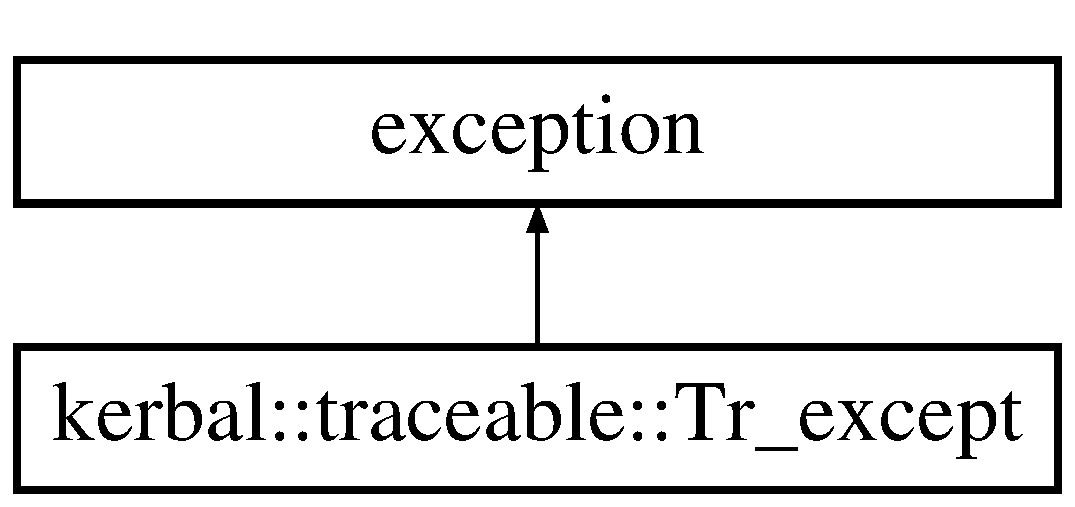
\includegraphics[height=2.000000cm]{classkerbal_1_1traceable_1_1_tr__except}
\end{center}
\end{figure}
\subsection*{类}
\begin{DoxyCompactItemize}
\item 
struct \hyperlink{structkerbal_1_1traceable_1_1_tr__except_1_1_trace}{Trace}
\end{DoxyCompactItemize}
\subsection*{Public 成员函数}
\begin{DoxyCompactItemize}
\item 
\mbox{\Hypertarget{classkerbal_1_1traceable_1_1_tr__except_a1f6b8bf28b4409c46120179d8650ba93}\label{classkerbal_1_1traceable_1_1_tr__except_a1f6b8bf28b4409c46120179d8650ba93}} 
{\bfseries Tr\+\_\+except} (const std\+::string \&\+\_\+\+M\+\_\+msg=\char`\"{}\char`\"{}, const std\+::string \&function\+\_\+name=\char`\"{}Unknown Function\char`\"{}, const std\+::string \&file\+\_\+name=\char`\"{}Unknown File\char`\"{}, int line=0)
\item 
\mbox{\Hypertarget{classkerbal_1_1traceable_1_1_tr__except_a7ff395a73c9b6721aa1847d2486239fc}\label{classkerbal_1_1traceable_1_1_tr__except_a7ff395a73c9b6721aa1847d2486239fc}} 
virtual const char $\ast$ {\bfseries what} () const \+\_\+\+G\+L\+I\+B\+C\+X\+X\+\_\+\+T\+X\+N\+\_\+\+S\+A\+F\+E\+\_\+\+D\+YN \+\_\+\+G\+L\+I\+B\+C\+X\+X\+\_\+\+U\+S\+E\+\_\+\+N\+O\+E\+X\+C\+E\+PT
\item 
\mbox{\Hypertarget{classkerbal_1_1traceable_1_1_tr__except_aa2fb4e5783dff16dbe387f9f42dcdfe0}\label{classkerbal_1_1traceable_1_1_tr__except_aa2fb4e5783dff16dbe387f9f42dcdfe0}} 
virtual void {\bfseries print\+\_\+trace} (std\+::ostream \&out=std\+::cerr) const
\item 
\mbox{\Hypertarget{classkerbal_1_1traceable_1_1_tr__except_af9315fa0298224e090578387935962be}\label{classkerbal_1_1traceable_1_1_tr__except_af9315fa0298224e090578387935962be}} 
virtual void {\bfseries re\+\_\+throw} (const std\+::string \&catch\+\_\+function\+\_\+name=\char`\"{}Unknown Function\char`\"{}, const std\+::string \&file\+\_\+name=\char`\"{}Unknown File\char`\"{}, int line=0) const
\end{DoxyCompactItemize}
\subsection*{Protected 属性}
\begin{DoxyCompactItemize}
\item 
\mbox{\Hypertarget{classkerbal_1_1traceable_1_1_tr__except_aef1f72279bbadc6f3cc6b8a9c36ec9ab}\label{classkerbal_1_1traceable_1_1_tr__except_aef1f72279bbadc6f3cc6b8a9c36ec9ab}} 
std\+::string {\bfseries \+\_\+\+M\+\_\+msg}
\item 
\mbox{\Hypertarget{classkerbal_1_1traceable_1_1_tr__except_a12f0843851f04e842237dd9852ce9fe6}\label{classkerbal_1_1traceable_1_1_tr__except_a12f0843851f04e842237dd9852ce9fe6}} 
std\+::list$<$ \hyperlink{structkerbal_1_1traceable_1_1_tr__except_1_1_trace}{Trace} $>$ {\bfseries trace\+\_\+record}
\end{DoxyCompactItemize}


该类的文档由以下文件生成\+:\begin{DoxyCompactItemize}
\item 
src/kerbal/Trexcept.\+hpp\item 
src/kerbal/Trexcept.\+cpp\end{DoxyCompactItemize}

\hypertarget{structkerbal_1_1traceable_1_1_tr__except_1_1_trace}{}\section{kerbal\+:\+:traceable\+:\+:Tr\+\_\+except\+:\+:Trace结构体 参考}
\label{structkerbal_1_1traceable_1_1_tr__except_1_1_trace}\index{kerbal\+::traceable\+::\+Tr\+\_\+except\+::\+Trace@{kerbal\+::traceable\+::\+Tr\+\_\+except\+::\+Trace}}
\subsection*{Public 成员函数}
\begin{DoxyCompactItemize}
\item 
\mbox{\Hypertarget{structkerbal_1_1traceable_1_1_tr__except_1_1_trace_aacad5214700c1ede35b8f040d396e415}\label{structkerbal_1_1traceable_1_1_tr__except_1_1_trace_aacad5214700c1ede35b8f040d396e415}} 
{\bfseries Trace} (std\+::string func\+\_\+name=\char`\"{}Unknown Function\char`\"{}, std\+::string file\+\_\+name=\char`\"{}Unknown File\char`\"{}, int line=0)
\end{DoxyCompactItemize}
\subsection*{Public 属性}
\begin{DoxyCompactItemize}
\item 
\mbox{\Hypertarget{structkerbal_1_1traceable_1_1_tr__except_1_1_trace_a4946f32b070a0bc288acfbe982154a0a}\label{structkerbal_1_1traceable_1_1_tr__except_1_1_trace_a4946f32b070a0bc288acfbe982154a0a}} 
std\+::string {\bfseries func\+\_\+name}
\item 
\mbox{\Hypertarget{structkerbal_1_1traceable_1_1_tr__except_1_1_trace_a8dbad22ac15fbae1c3d8bd8d03520572}\label{structkerbal_1_1traceable_1_1_tr__except_1_1_trace_a8dbad22ac15fbae1c3d8bd8d03520572}} 
std\+::string {\bfseries file\+\_\+name}
\item 
\mbox{\Hypertarget{structkerbal_1_1traceable_1_1_tr__except_1_1_trace_a11bd6453d09569ee05832e73b45507d0}\label{structkerbal_1_1traceable_1_1_tr__except_1_1_trace_a11bd6453d09569ee05832e73b45507d0}} 
int {\bfseries line}
\end{DoxyCompactItemize}


该结构体的文档由以下文件生成\+:\begin{DoxyCompactItemize}
\item 
src/kerbal/Trexcept.\+hpp\end{DoxyCompactItemize}

\chapter{文件说明}
\hypertarget{matrix_8hpp}{}\section{src/kerbal/math/matrix.hpp 文件参考}
\label{matrix_8hpp}\index{src/kerbal/math/matrix.\+hpp@{src/kerbal/math/matrix.\+hpp}}


本文件提供了对基本矩阵计算的支持  


{\ttfamily \#include $<$fstream$>$}\newline
{\ttfamily \#include $<$iostream$>$}\newline
{\ttfamily \#include $<$cmath$>$}\newline
{\ttfamily \#include \char`\"{}../array\+\_\+2d.\+hpp\char`\"{}}\newline
\subsection*{类}
\begin{DoxyCompactItemize}
\item 
class \hyperlink{classkerbal_1_1math_1_1_matrix}{kerbal\+::math\+::\+Matrix}
\begin{DoxyCompactList}\small\item\em 矩阵类 \end{DoxyCompactList}\end{DoxyCompactItemize}
\subsection*{命名空间}
\begin{DoxyCompactItemize}
\item 
 \hyperlink{namespacekerbal}{kerbal}
\begin{DoxyCompactList}\small\item\em kerbal 库 \end{DoxyCompactList}\item 
 \hyperlink{namespacekerbal_1_1math}{kerbal\+::math}
\begin{DoxyCompactList}\small\item\em 数学计算子库 \end{DoxyCompactList}\end{DoxyCompactItemize}
\subsection*{函数}
\begin{DoxyCompactItemize}
\item 
void {\bfseries std\+::swap} (\hyperlink{classkerbal_1_1math_1_1_matrix}{kerbal\+::math\+::\+Matrix} \&a, \hyperlink{classkerbal_1_1math_1_1_matrix}{kerbal\+::math\+::\+Matrix} \&b)
\begin{DoxyCompactList}\small\item\em 交换两个矩阵 \end{DoxyCompactList}\item 
\mbox{\Hypertarget{namespacekerbal_1_1math_aac8c0ee9511d7ac59fdca86e0d7a5ef9}\label{namespacekerbal_1_1math_aac8c0ee9511d7ac59fdca86e0d7a5ef9}} 
{\footnotesize template$<$size\+\_\+t N$>$ }\\const Matrix {\bfseries kerbal\+::math\+::cat} (const Matrix(\&a)\mbox{[}N\mbox{]})  throw (std\+::invalid\+\_\+argument)
\item 
\mbox{\Hypertarget{namespacekerbal_1_1math_ab0c3317760651c36ccae631e6826ff32}\label{namespacekerbal_1_1math_ab0c3317760651c36ccae631e6826ff32}} 
const Matrix {\bfseries kerbal\+::math\+::rotate\+\_\+X} (double sigma)
\item 
\mbox{\Hypertarget{namespacekerbal_1_1math_a8ae35ffad8d30503414300f7461e50d6}\label{namespacekerbal_1_1math_a8ae35ffad8d30503414300f7461e50d6}} 
const Matrix {\bfseries kerbal\+::math\+::rotate\+\_\+Y} (double sigma)
\item 
\mbox{\Hypertarget{namespacekerbal_1_1math_a4380bab6442decaf30f51695058e42da}\label{namespacekerbal_1_1math_a4380bab6442decaf30f51695058e42da}} 
const Matrix {\bfseries kerbal\+::math\+::rotate\+\_\+Z} (double sigma)
\item 
\mbox{\Hypertarget{namespacekerbal_1_1math_a37e3d41de6613f1820954b46fc431762}\label{namespacekerbal_1_1math_a37e3d41de6613f1820954b46fc431762}} 
void {\bfseries kerbal\+::math\+::rotate\+\_\+X} (double sigma, const double \&x0, double \&y0, double \&z0)  throw ()
\item 
\mbox{\Hypertarget{namespacekerbal_1_1math_a128fd0aa8828144d753d6d000dba8406}\label{namespacekerbal_1_1math_a128fd0aa8828144d753d6d000dba8406}} 
void {\bfseries kerbal\+::math\+::rotate\+\_\+Y} (double sigma, double \&x0, const double \&y0, double \&z0)  throw ()
\item 
\mbox{\Hypertarget{namespacekerbal_1_1math_ae2c2044405fa1e952ccb07dae1a61111}\label{namespacekerbal_1_1math_ae2c2044405fa1e952ccb07dae1a61111}} 
void {\bfseries kerbal\+::math\+::rotate\+\_\+Z} (double sigma, double \&x0, double \&y0, const double \&z0)  throw ()
\end{DoxyCompactItemize}


\subsection{详细描述}
本文件提供了对基本矩阵计算的支持 

\begin{DoxyAuthor}{作者}
倪文卿 
\end{DoxyAuthor}
\begin{DoxyDate}{日期}
2017-\/4-\/30 
\end{DoxyDate}
\begin{DoxyCopyright}{版权所有}
倪文卿 

\href{http://thinkspirit.org/}{\tt Think\+Spirit Laboratory} of \href{http://www.nuist.edu.cn/}{\tt Nanjing University of Information Science \& Technology}  
\end{DoxyCopyright}


\subsection{函数说明}
\mbox{\Hypertarget{matrix_8cpp_file_abf53e915d879b9a0ba35b7d3e6fd6f8b}\label{matrix_8cpp_file_abf53e915d879b9a0ba35b7d3e6fd6f8b}} 
\index{matrix.\+hpp@{matrix.\+hpp}!swap@{swap}}
\index{swap@{swap}!matrix.\+hpp@{matrix.\+hpp}}
\subsubsection{\texorpdfstring{swap()}{swap()}}
{\footnotesize\ttfamily void std\+::swap (\begin{DoxyParamCaption}\item[{\hyperlink{classkerbal_1_1math_1_1_matrix}{kerbal\+::math\+::\+Matrix} \&}]{a,  }\item[{\hyperlink{classkerbal_1_1math_1_1_matrix}{kerbal\+::math\+::\+Matrix} \&}]{b }\end{DoxyParamCaption})}



交换两个矩阵 


\begin{DoxyParams}{参数}
{\em a} & 矩阵 a \\
\hline
{\em b} & 矩阵 b \\
\hline
\end{DoxyParams}
\begin{DoxyRemark}{备注}
重载了标准命名空间中的 swap 函数, 使得两个矩阵的交换操作能在 O(1) 的时间复杂度中完成 
\end{DoxyRemark}

%--- End generated contents ---

% Index
\backmatter
\newpage
\phantomsection
\clearemptydoublepage
\addcontentsline{toc}{chapter}{索引}
\printindex

\end{document}
